Во второй главе рассматривается, каким образом требования, сформулированные в первой
главе, переводятся в реализованную систему управления контентом на базе
\texttt{Strapi} и \texttt{Astro}. Если в аналитической части были зафиксированы
необходимость независимого редакторского цикла, структурированной модели данных,
локализованной витрины \texttt{ru/en}, управляемых метаданных, \texttt{preview} и
воспроизводимой публикации, то далее показывается, как эти требования закреплены в
архитектуре приложений, модели данных \texttt{CMS}, page builder-контуре и
frontend-слое.

Описание опирается только на те решения, которые подтверждаются структурой
репозитория, конфигурацией приложений, схемами контентных типов, маршрутами
frontend-части и реализованными пользовательскими сценариями. Поэтому глава
выстроена в последовательности ``архитектура -> данные -> \texttt{Dynamic Zone} ->
публичная витрина -> эксплуатационные контуры'': сначала фиксируется общий
\texttt{CMS-first} каркас, затем раскрывается, как он превращается в управляемые
контентные сущности, в конструктор страниц и в опубликованный storefront. Такой
порядок позволяет рассматривать проектную главу не как план развития системы, а как
описание уже существующего инженерного контура управления маркетинговым контентом.

\section{Общая архитектура системы}

\subsection{Структура репозитория и роли приложений}

Проект реализован как монорепозиторий \texttt{Nx + pnpm}, поскольку в рамках
\texttt{CMS-first} системы контентная схема, \texttt{API}-контракт, frontend-рендеринг
и публикационный контур изменяются совместно. В составе репозитория выделены два
самостоятельных приложения: \texttt{apps/cms} на \texttt{Strapi 5} и
\texttt{apps/front} на \texttt{Astro 6}. Для каждого из них определены собственные
\texttt{Nx}-цели разработки, сборки и проверки, поэтому \texttt{CMS} и публичная
витрина сопровождаются как независимые исполняемые контуры, но остаются в одной кодовой
базе. Практический эффект такого решения состоит в том, что изменение модели данных,
маршрутов или публикационного механизма можно проводить атомарно, без рассинхронизации
между backend и frontend.

С архитектурной точки зрения \texttt{Strapi} выступает ядром редакторской части
системы. В нем сосредоточены контентные типы, отношения между сущностями,
локализуемые поля, режим \texttt{draft/publish}, роли и публичный \texttt{REST API}.
\texttt{Astro}, напротив, выполняет роль слоя публикации: получает данные из
\texttt{CMS}, формирует маршруты витрины, рендерит страницы и обслуживает
\texttt{preview}-сценарии. Тем самым разделение, обоснованное в первой главе,
становится реализованной архитектурой: контент управляется в \texttt{CMS}, а публичное
представление строится в отдельном frontend-контуре.

Интеграция между этими приложениями организована в двух взаимодополняющих формах.
Во-первых, \texttt{Strapi} публикует OpenAPI-описание, а во frontend используется
генерация типизированного клиента, что снижает риск расхождения между маршрутами
backend и потребителями данных. Во-вторых, для \texttt{global}, \texttt{home-page},
\texttt{page} и карьерного модуля сохранен отдельный слой доступа к данным с явным
управлением локалями, \texttt{populate}-параметрами и \texttt{preview}-режимом. Такое
сочетание не является дублированием: типизированный клиент удобен для стабильных
коллекционных сценариев, тогда как page builder- и \texttt{preview}-контуры требуют
более точного контроля над составом загружаемых данных. Сводно архитектура системы
показана на рисунке~\ref{fig:chapter2-cms-first-architecture} в приложении~А.

\subsection{Контур доставки контента}

Контур доставки контента реализует центральное требование первой главы: публичная
витрина должна зависеть от управляемых данных \texttt{CMS}, а не от ручной правки
шаблонов. Для этого в системе закреплена схема \texttt{Strapi -> API -> Astro}:
контент создается и проходит публикационный жизненный цикл в \texttt{Strapi}, после
чего frontend запрашивает уже опубликованные данные и использует их для формирования
публичных страниц. Для \texttt{home-page}, \texttt{page}, а также для разделов
\texttt{articles} и \texttt{projects} эта схема реализована в locale-prefixed
маршрутах, тогда как карьерный модуль \texttt{vacancies} публикуется как отдельный
прикладной контур с маршрутами \texttt{/vacancies/} и \texttt{/vacancies/:slug/}. Тем
самым маршрутная граница витрины следует принятому scope: storefront-core строится как
двуязычный маркетинговый контур, а кадровый сценарий сохраняет собственную публичную
поверхность при общей \texttt{CMS}-модели данных.

На стороне frontend этот подход поддерживается конфигурацией \texttt{Astro}: подключены
адаптер \texttt{Node.js}, модуль \texttt{sitemap} и абсолютный \texttt{site}-контракт
через переменные окружения. Итоговая сборка формируется в standalone-режиме и служит
основой для отдельного \texttt{Docker}-приложения витрины, которое далее разворачивается
в \texttt{Dokploy}. При этом базовый режим работы остается статически ориентированным:
основные публичные маршруты публикуются как заранее подготовленный результат, а
server-side логика используется только там, где она действительно нужна, прежде всего
для \texttt{preview}. Практический эффект заключается в предсказуемой публикации
контента: \texttt{CMS} управляет данными и событиями публикации, а витрина отдает уже
сформированное представление.

\section{Проектирование модели данных CMS}

\subsection{Сущности, атрибуты и связи}

Модель данных \texttt{CMS} выступает тем уровнем, на котором требования главы~1
превращаются в формализованные управляемые сущности. Вместо одного универсального
``страничного'' типа в \texttt{Strapi} разделены несколько контуров: редакционный
маркетинговый контент, карьерный прикладной контур, глобальные данные витрины и записи,
возникающие в результате действий внешнего пользователя. Поэтому в системе определены
коллекции \texttt{article}, \texttt{author}, \texttt{project}, \texttt{vacancy},
\texttt{vacancy-application}, \texttt{lead-submission}, \texttt{industry},
\texttt{job-role} и \texttt{page}, а также single type-сущности \texttt{global} и
\texttt{home-page}. Такой набор отражает не структуру отдельных шаблонов, а состав
предметной области, которой должен управлять редактор.

Редакционный контур охватывает прежде всего \texttt{page}, \texttt{home-page},
\texttt{article}, \texttt{author} и \texttt{project}. Он отвечает за страницы витрины,
публикации и кейсы, то есть за сущности, для которых критичны локализуемые
\texttt{slug}, rich text-контент, media-атрибуты и управляемый жизненный цикл
публикации. Карьерный контур организован вокруг \texttt{vacancy}, \texttt{industry} и
\texttt{job-role}: в \texttt{vacancy} зафиксированы не только заголовок и описание, но
и прикладные атрибуты кадрового сценария, включая связь с отраслью и ролью, формат
работы, тип занятости, уровень и зарплатные диапазоны. Практический эффект такого
разделения состоит в том, что маркетинговый и кадровый сценарии используют общее
\texttt{CMS}-ядро, но не смешивают свои типы контента и правила его сопровождения.

Отдельный слой образуют прикладные записи, создаваемые не редактором, а пользователем
витрины. Сущность \texttt{vacancy-application} хранит ссылку на вакансию, персональные
данные кандидата, файл резюме, отметку согласия, момент отправки, источник и внутренний
\texttt{HR}-статус. Сущность \texttt{lead-submission}, в свою очередь, обслуживает
маркетинговый сценарий и сохраняет имя, email, телефон, компанию, текст запроса,
\texttt{submittedAt}, идентификатор формы, путь и заголовок страницы, а также локаль
отправки. За счет этого \texttt{CMS} используется не только как хранилище страниц и
публикаций, но и как единая точка фиксации прикладных результатов работы витрины.

На уровне связей модель включает отношение \texttt{manyToMany} между статьями и
авторами, отношение \texttt{manyToOne} от вакансии к отрасли и роли, а также отношение
\texttt{manyToOne} от отклика к вакансии. Для \texttt{article}, \texttt{author},
\texttt{project}, \texttt{vacancy}, \texttt{industry}, \texttt{job-role},
\texttt{global}, \texttt{home-page} и \texttt{page} включены \texttt{draft/publish} и
\texttt{i18n}, поскольку для этих сущностей требуется редакторская подготовка, локали
\texttt{ru/en} и раздельные состояния черновика и публикации. Для
\texttt{vacancy-application} и \texttt{lead-submission} такие механизмы намеренно не
используются: эти записи фиксируют факт отправки формы, а не объект редакторского
контроля. Следовательно, сама структура модели данных уже проводит границу между
управляемым контентом и прикладными событиями. Сводная модель сущностей и их связей
приведена на рисунке~\ref{fig:chapter2-cms-data-model} в приложении~Б, а жизненный цикл
локализуемой контентной единицы с режимом \texttt{draft/publish} --- на
рисунке~\ref{fig:chapter2-cms-content-lifecycle} в приложении~В.

\subsection{\texttt{SEO}-модель и глобальные сущности}

Важную роль в этой модели играют две single type-сущности: \texttt{global} и
\texttt{home-page}. Первая закрывает требование о \texttt{CMS}-управляемых общих данных
витрины: в \texttt{global} вынесены название компании, описание, логотип, навигация,
primary и secondary \texttt{CTA}, колонки футера и копирайт. Благодаря этому layout
уровня \texttt{Header/Footer} перестает зависеть от локальных frontend-констант и
получает тот же редакторский статус, что и основной контент страницы.

Сущность \texttt{home-page} решает другую архитектурную задачу: главная страница
включается в ту же управляемую модель, что и обычные \texttt{page}-страницы. Она хранит
описание, набор блоков и вложенный \texttt{SEO}-компонент, поэтому главная витрина
редактируется не как исключение в коде, а как самостоятельная запись в \texttt{CMS}.
Далее эта логика расширяется на единый \texttt{SEO}-контур: компонент
\texttt{shared.seo} используется не только в \texttt{home-page} и \texttt{page}, но и
в сущностях \texttt{article}, \texttt{project} и \texttt{vacancy}. Он задает
\texttt{metaTitle}, \texttt{metaDescription}, \texttt{canonicalURL}, поля
\texttt{Open Graph}, изображение для предпросмотра и признак \texttt{noIndex}. В
результате frontend получает один и тот же контракт метаданных для главной страницы,
маркетинговых \texttt{slug}-страниц и ключевых детальных сущностей. Практический эффект
состоит в том, что витрина может строить \texttt{SEO}-слой централизованно, не
дублируя схему метаданных в каждом типе маршрута.

\section{Конструктор страниц на основе \texttt{Dynamic Zone}}

\subsection{Сущность \texttt{page} и набор блоков}

Коллекция \texttt{page} выступает основным редакторским интерфейсом для независимой
сборки маркетинговых страниц. Каждая запись объединяет локализуемый \texttt{slug},
\texttt{SEO}-метаданные и массив блоков, а структура страницы хранится не в route-файле
frontend, а в \texttt{Dynamic Zone} на стороне \texttt{CMS}. Именно здесь требование
первой главы о редактировании типовой маркетинговой страницы без правки frontend-кода
получает практическую реализацию: редактор меняет не только тексты, но и композицию
страницы как часть одной сущности.

Для \texttt{page} и \texttt{home-page} используется единая библиотека блоков, в которую
входят \texttt{hero}, \texttt{rich-text}, \texttt{feature-cards}, \texttt{cta},
\texttt{preview-list}, \texttt{logo-cloud}, \texttt{testimonials}, \texttt{stats},
\texttt{feature-highlight}, \texttt{faq}, \texttt{process-timeline}, \texttt{quote},
\texttt{checklist}, \texttt{content-columns}, \texttt{numbered-points} и
\texttt{lead-form}. Блоки оформлены как отдельные \texttt{Strapi}-компоненты и
используют вложенные shared-компоненты для карточек, ссылок, \texttt{FAQ}-элементов,
шагов процесса, статистики и других переиспользуемых частей модели данных. Такое
решение переводит page builder из набора одноразовых секций в устойчивый словарь
редакторских конструкций, одинаково применимый к главной и внутренним маркетинговым
страницам.

Особенно показателен блок \texttt{lead-form}: он задает не только визуальную секцию, но
и поля прикладного сценария, включая имя формы, тексты согласия и сообщения после
отправки. За счет этого page builder охватывает не только презентационную, но и
конверсионную функцию витрины. Практически такой редакторский контур виден на
рисунке~\ref{fig:chapter2-page-editor}: в одной сущности одновременно задаются
\texttt{slug}, последовательность блоков, \texttt{SEO}-поля и точка входа в
\texttt{preview}-сценарий.

\begin{figure}[htbp]
  \centering
  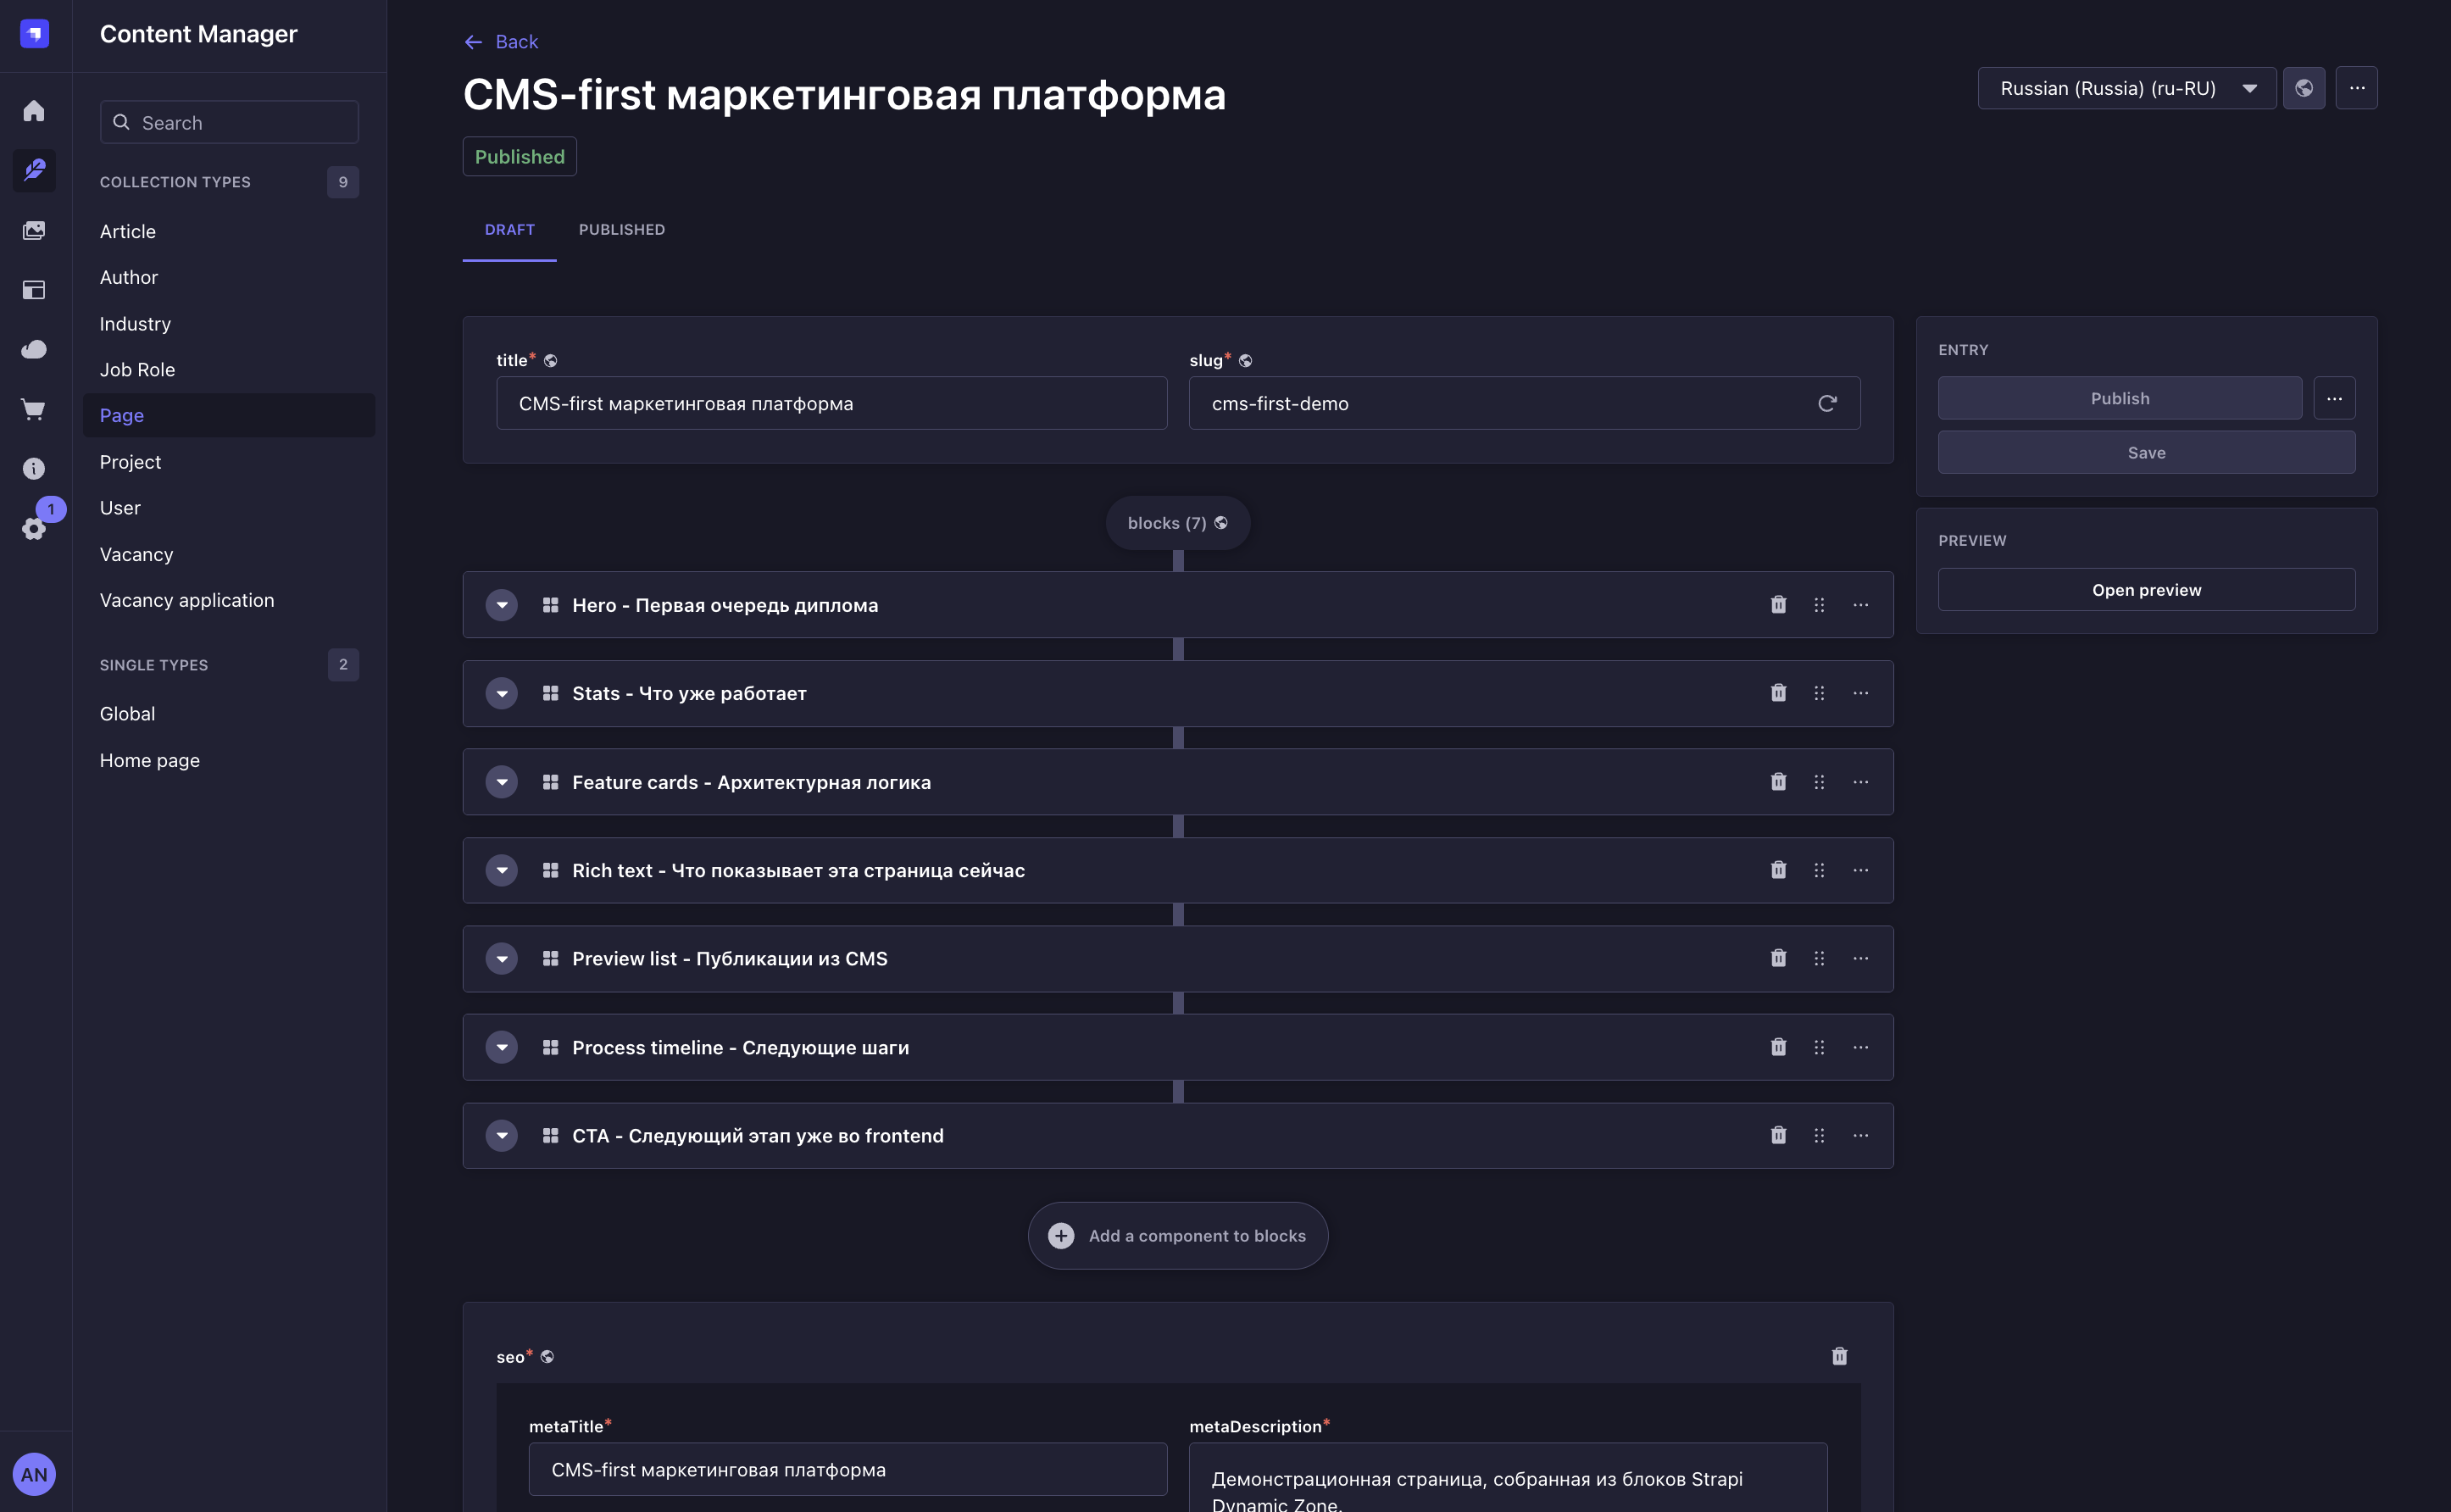
\includegraphics[width=\linewidth]{assets/strapi-images/page.png}
  \caption{Редактирование CMS-страницы в \texttt{Strapi}: \texttt{slug}, \texttt{Dynamic Zone}, \texttt{SEO} и доступ к \texttt{preview}}
  \label{fig:chapter2-page-editor}
\end{figure}

\subsection{Связь CMS-блоков с frontend-рендерингом}

На стороне frontend \texttt{Dynamic Zone} поддерживается общим renderer-слоем, который
принимает массив блоков и передает каждый элемент в специализированный компонент на
\texttt{Astro} или \texttt{React}. Тем самым frontend не содержит ручного описания
конкретной маркетинговой страницы: route-файл отвечает только за получение записи,
маршрутный контекст и метаданные, а фактическая композиция страницы определяется
данными \texttt{CMS}. Это и делает page builder полноценным механизмом публикации, а не
только удобством админ-панели.

Практический эффект такого маппинга особенно заметен в двух случаях. Для блока
\texttt{preview-list} реализована связка с разделами \texttt{articles},
\texttt{projects} и \texttt{vacancies}, поэтому \texttt{CMS}-страница может включать
динамические анонсы существующих коллекций без отдельной ручной раскладки в шаблоне.
Для блока \texttt{lead-form} frontend дополнительно передает путь, заголовок и локаль
текущей страницы, что позволяет сохранять маркетинговый лид вместе с контекстом его
происхождения. Следовательно, \texttt{Dynamic Zone} связывает модель данных с реальным
пользовательским поведением витрины, а не ограничивается текстовым наполнением секций.

\section{Реализация frontend-части на \texttt{Astro}}

\subsection{Локализованные маршруты главной и CMS-страниц}

Локализованный маршрутный слой frontend является прямым продолжением \texttt{CMS}-модели
данных. Для главной страницы используются маршруты \texttt{/ru/} и \texttt{/en/}, для
\texttt{page} --- маршруты вида \texttt{/:locale/:slug/}, а корневой адрес
\texttt{/} выполняет редирект на \texttt{/ru/} как на базовую точку входа в витрину.
Во время сборки frontend получает из \texttt{CMS} список локалей и набор доступных
\texttt{slug} для каждой локали, после чего route-файлы формируют локализованный путь,
\texttt{SEO}-метаданные и передают массив блоков в общий renderer. Тем самым адрес,
контент и метаинформация страницы выводятся из одной и той же записи \texttt{CMS}, а не
собираются из разрозненных frontend-констант.

С инженерной точки зрения это означает, что главная витрина и маркетинговые
\texttt{slug}-страницы уже работают как единый \texttt{CMS-first} storefront: появление
или изменение страницы определяется публикацией записи в \texttt{Strapi}, а не созданием
нового route-файла. Такой способ построения multilingual route-контура соответствует как
встроенной \texttt{i18n}-модели \texttt{Astro}, так и рекомендациям по публикации
локализованных версий страниц для поисковых систем~\cite{astro-i18n-routing,google-international-sites}.
На рисунке~\ref{fig:chapter2-home-en-route} показана английская версия главной страницы
по маршруту \texttt{/en/}; тот же принцип locale-prefixed адресации используется и для
управляемых \texttt{CMS}-страниц с маршрутами вида \texttt{/:locale/:slug/}.

\begin{figure}[htbp]
  \centering
  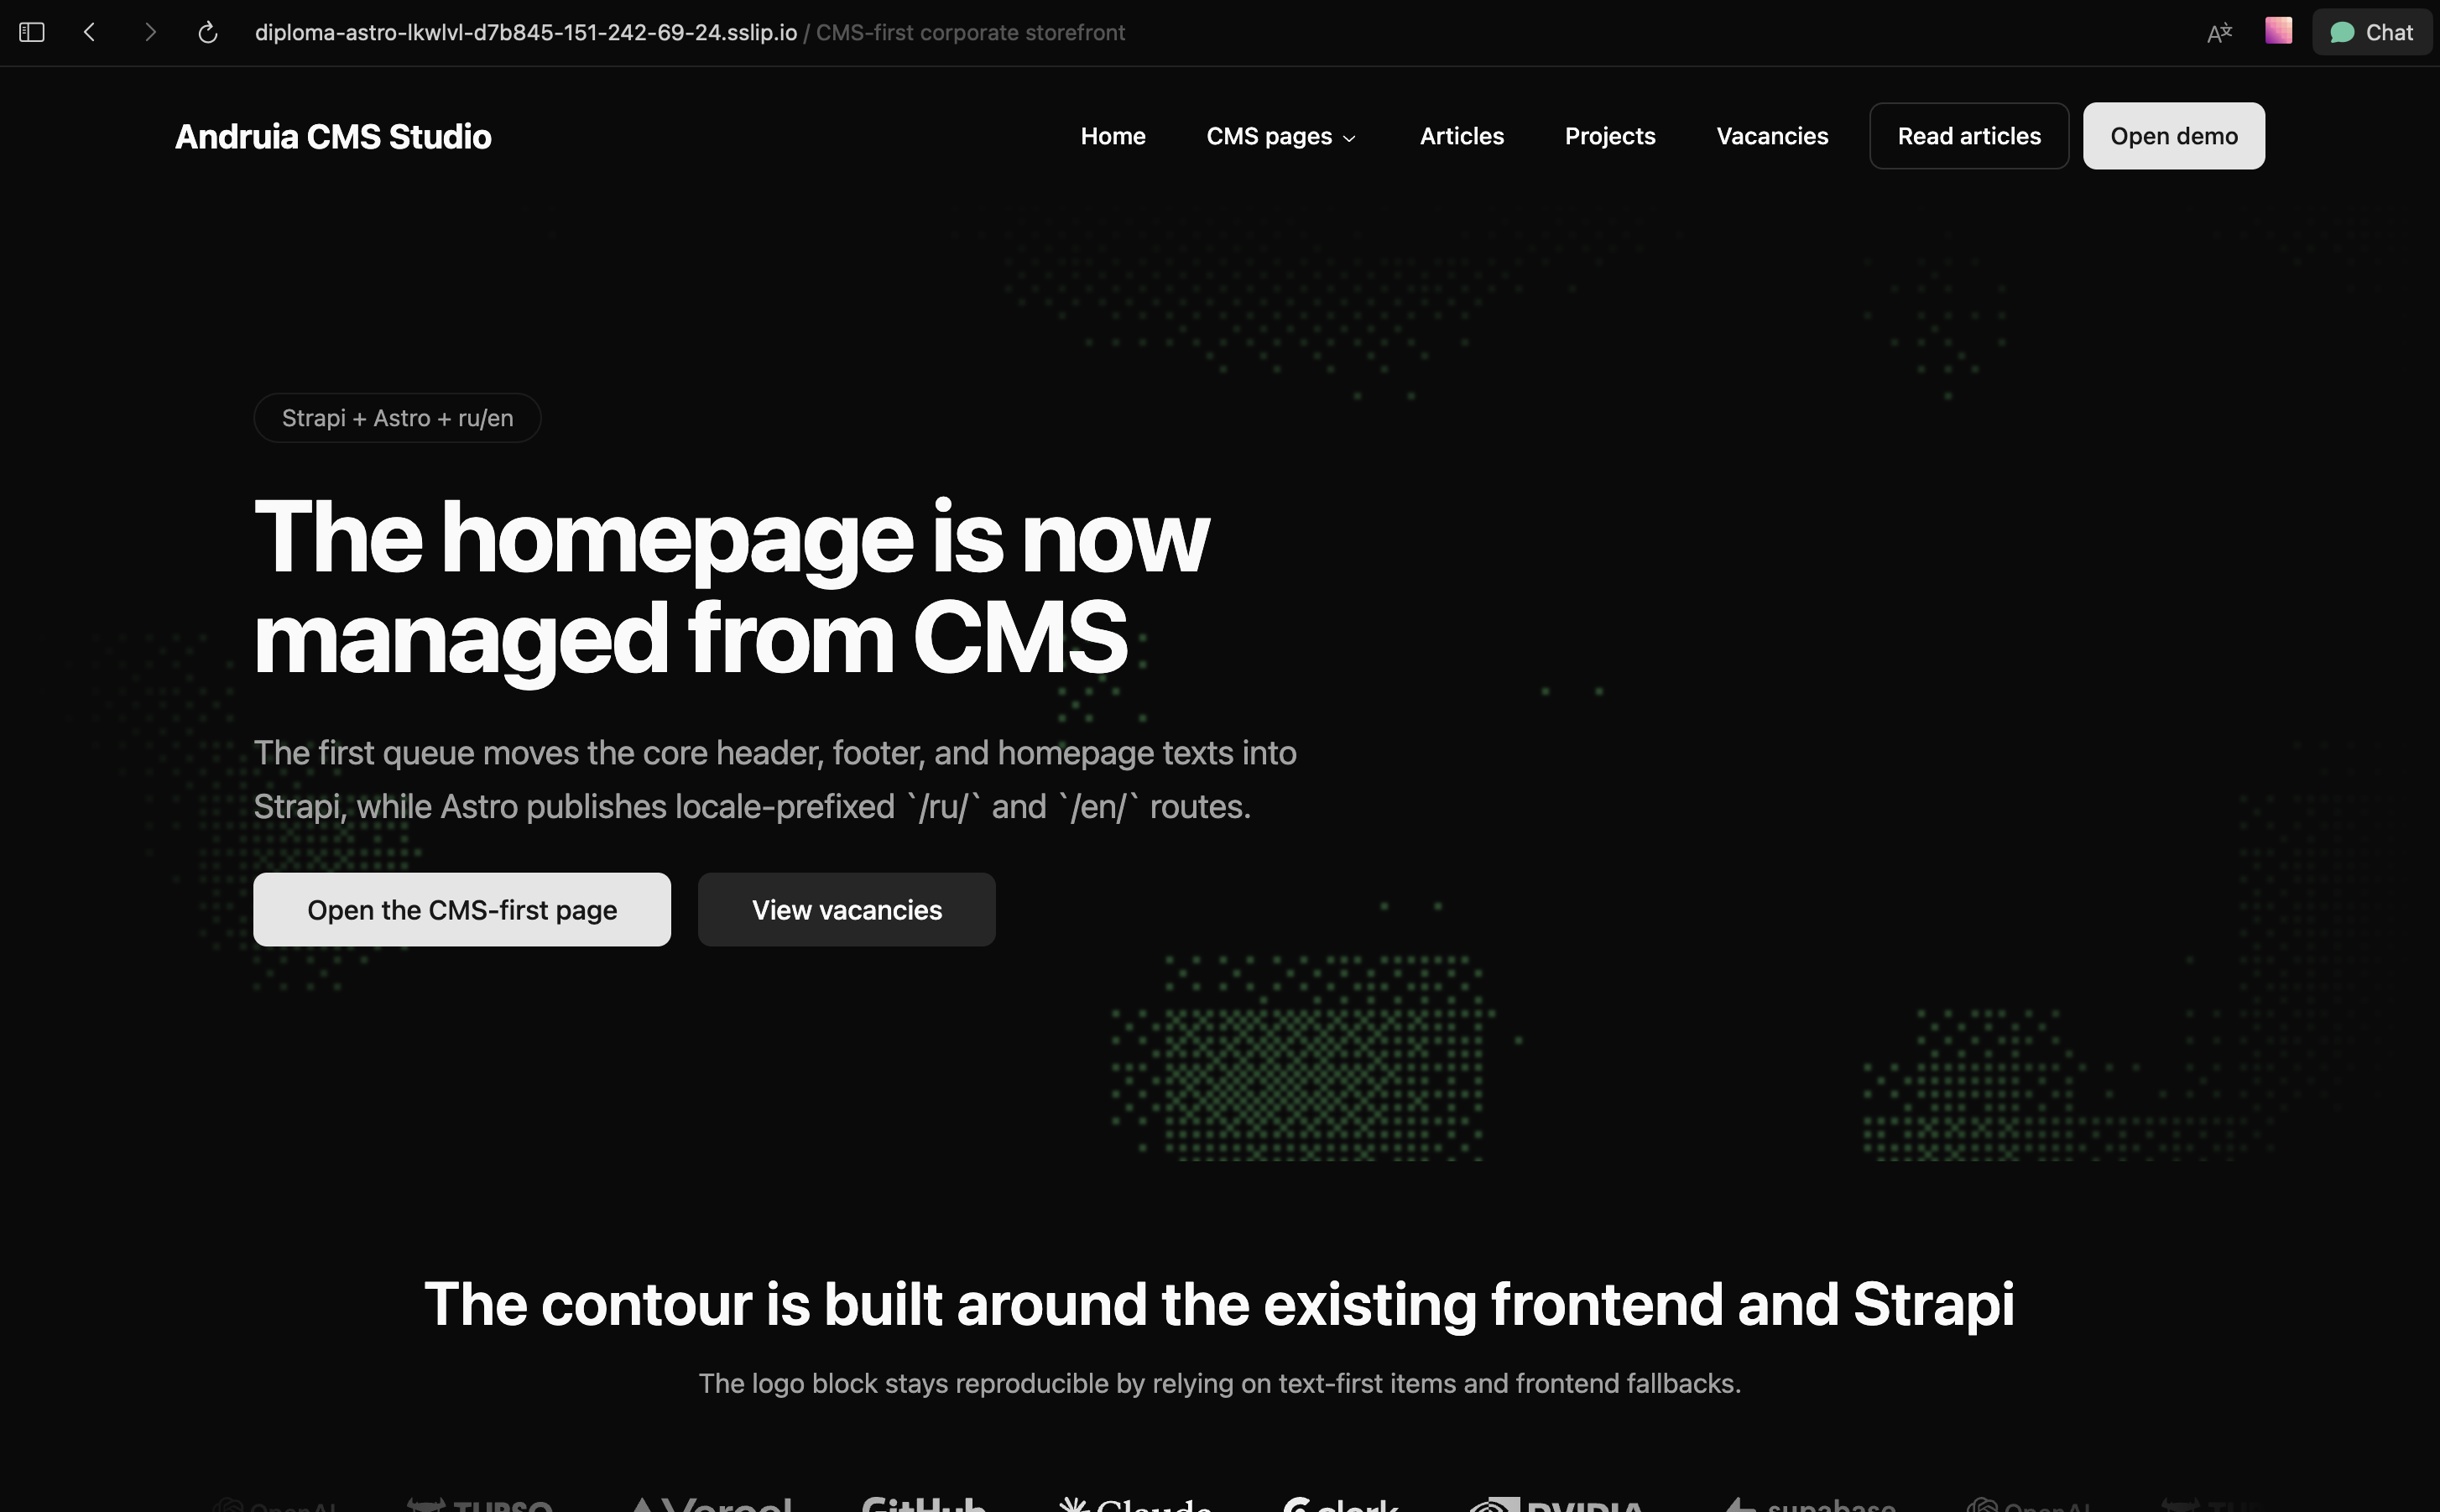
\includegraphics[width=\linewidth]{assets/front/home-en-with-url.png}
  \caption{Публичная витрина в locale-prefixed маршруте \texttt{/en/}, опубликованная на основе данных из CMS}
  \label{fig:chapter2-home-en-route}
\end{figure}

\subsection{Статьи, проекты и карьерный модуль}

Frontend не ограничивается page builder-маршрутами и тем самым завершает превращение
\texttt{CMS} из хранилища страниц в источник всей публичной витрины. Для
\texttt{articles} и \texttt{projects} реализованы отдельные коллекционные разделы,
встроенные в locale-prefixed схему \texttt{/:locale/articles/...} и
\texttt{/:locale/projects/...}. Списковые страницы этих разделов используют
сгенерированный типизированный клиент, а детальные страницы загружают полную сущность по
\texttt{slug}. Практический эффект такого решения состоит в том, что одна и та же
\texttt{CMS}-модель обеспечивает как произвольные маркетинговые страницы, так и
повторяемые редакционные форматы публикаций и кейсов внутри общего storefront-контура.

Карьерный модуль, напротив, реализован как отдельный прикладной маршрутный слой.
Каталог использует \texttt{VacancyExplorer} с фильтрацией по отрасли, роли, локации,
формату работы, типу занятости и уровню, а детальная страница вакансии отображает
атрибуты записи и подключает форму отклика. Тем самым frontend обслуживает уже не только
редакционные материалы, но и кадровый пользовательский сценарий, в котором
\texttt{Strapi} остается источником данных как для самих вакансий, так и для связанных
таксономий. Соответствующая публичная точка взаимодействия показана на
рисунке~\ref{fig:chapter2-vacancy-detail}: детальная страница одновременно отображает
данные вакансии и форму, которая затем передает отклик в \texttt{vacancy-application}.
Важно, что в итоговом дипломном scope это трактуется не как незавершенная локализация, а
как отдельный прикладной публичный контур: локализация вакансий, отраслей и ролей
сохраняется в модели данных и в \texttt{preview}, тогда как production-маршруты
кадрового сценария осознанно остаются под \texttt{/vacancies/*}.

\begin{figure}[H]
  \centering
  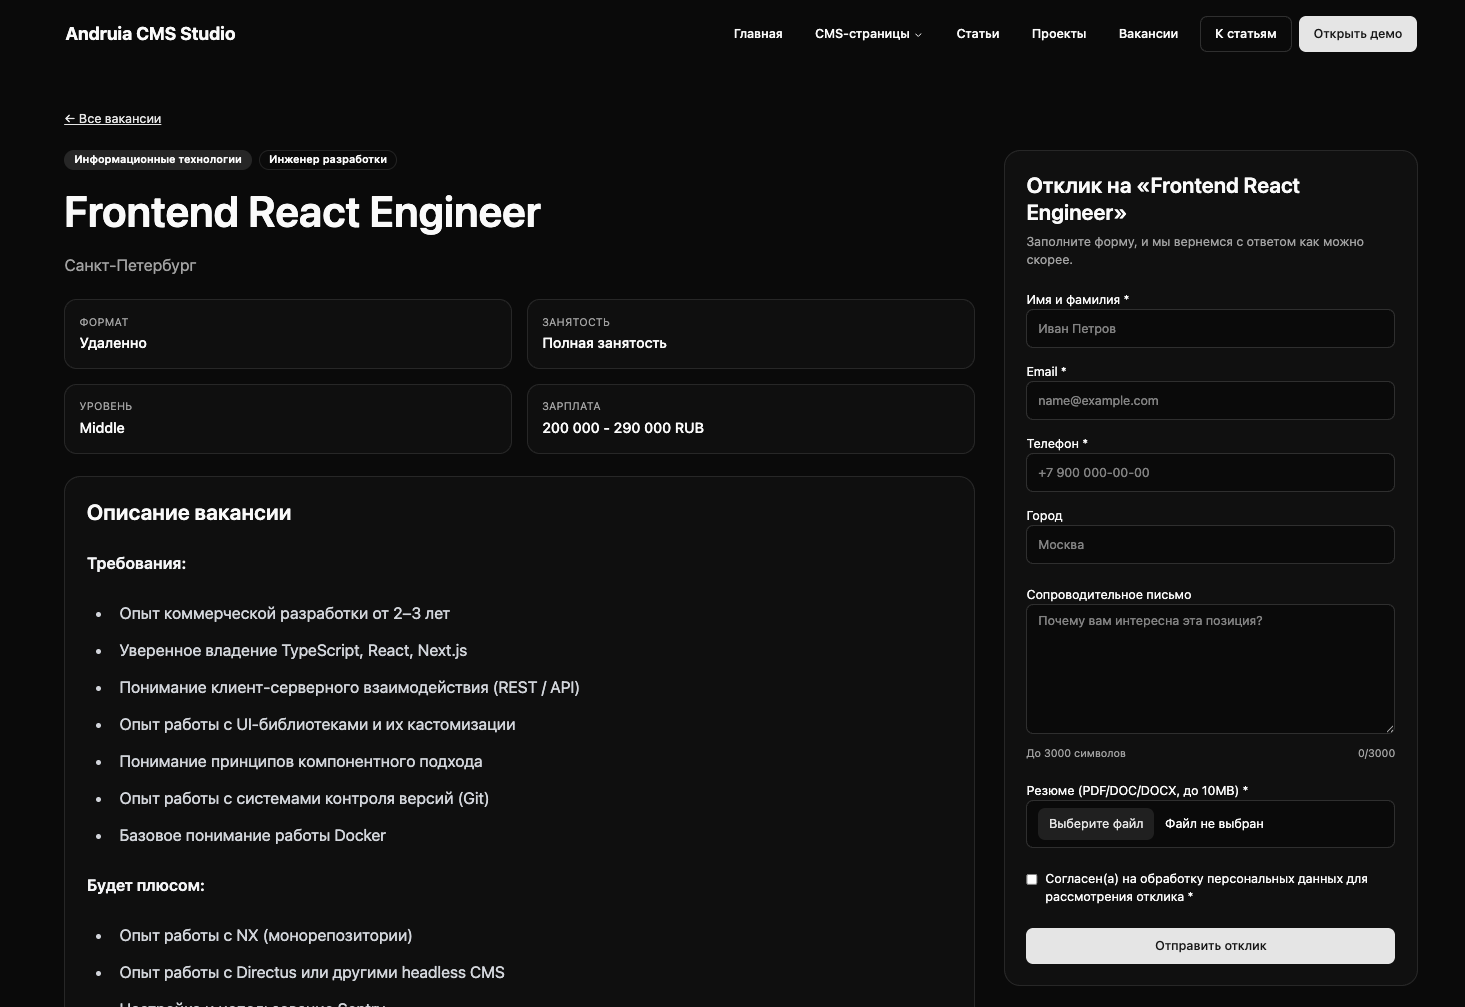
\includegraphics[width=\linewidth]{assets/front/frontend-vacancy.png}
  \caption{Детальная страница вакансии с подключенной формой отклика как прикладной публичный сценарий}
  \label{fig:chapter2-vacancy-detail}
\end{figure}

Отдельно от карьерного сценария реализован маркетинговый прикладной контур для
\texttt{home-page} и \texttt{page}. Если редактор добавляет в \texttt{Dynamic Zone}
блок \texttt{lead-form}, frontend рендерит встроенную форму, валидирует ее на клиенте и
затем передает данные в server-side маршрут \texttt{/api/lead-submissions}. Этот маршрут
повторно проверяет payload, применяет \texttt{honeypot} и создает запись
\texttt{lead-submission} в \texttt{Strapi} через server-side \texttt{API token}. За счет
этого page builder доводится до полного практического цикла: \texttt{CMS} определяет не
только состав секций страницы, но и сценарий получения маркетингового лида с сохранением
контекста страницы и локали.

Таким образом, первая половина проектной главы выстраивает непрерывную линию от
архитектурного разделения \texttt{Strapi} и \texttt{Astro} к предметной модели данных,
затем к \texttt{Dynamic Zone} как редакторскому механизму сборки страницы и далее к
frontend как к слою публикации этого контента в виде публичной витрины. На этой основе
дальнейшие разделы главы уже раскрывают сквозные свойства системы --- мультиязычность,
\texttt{preview}, \texttt{SEO} и публикационный контур --- как продолжение уже
сформированной архитектурной логики, а не как набор изолированных функций.

\section{Мультиязычность}

\subsection{Локали в модели данных и в маршрутизации}

Поддержка мультиязычности в проекте реализована как часть общей архитектуры данных и
маршрутов. Во frontend зафиксированы две публичные локали: \texttt{ru} и \texttt{en}.
Для них определено отображение в локали CMS: \texttt{ru -> ru-RU}, \texttt{en -> en}. На
уровне \texttt{Strapi} локализация включена для ключевых контентных сущностей, включая
\texttt{page}, \texttt{home-page}, \texttt{global}, \texttt{article}, \texttt{project},
\texttt{vacancy}, \texttt{author}, \texttt{industry} и \texttt{job-role}. Это позволяет
хранить локализованные значения контента, \texttt{slug} и связанных полей непосредственно
в CMS.

Витрина использует эти локали в двух местах. Во-первых, они участвуют в генерации
locale-prefixed маршрутов для главной витрины, CMS-страниц, а также разделов статей и
проектов. Во-вторых, они передаются в layout, который вычисляет корректный
\texttt{lang}-атрибут HTML-документа, canonical URL и локаль для \texttt{Open Graph}.
Таким образом, мультиязычность проявляется не только как свойство контентных полей, но
и как часть публичного маршрутного контура для главной витрины и CMS-страниц.

Для карьерного модуля мультиязычность проведена по другой, но согласованной границе.
Сущности \texttt{vacancy}, \texttt{industry} и \texttt{job-role} локализуются в
\texttt{Strapi}, а \texttt{preview}-контур вакансий принимает явную локаль и обращается к
соответствующей версии записи. Однако production-публикация карьерного сценария не
переводится в обязательный locale-prefixed контур \texttt{/:locale/vacancies/...}. В
рамках данной ВКР это рассматривается как осознанное разделение между multilingual
storefront-core и отдельным прикладным кадровым модулем, а не как дефект архитектуры.

\subsection{CMS-управляемые глобальные данные}

Дополнительным результатом реализованного решения является вынос ключевых UI-текстов витрины
в \texttt{Strapi}. Layout запрашивает сущность \texttt{global} с учетом активной локали,
после чего передает в компоненты \texttt{Header} и \texttt{Footer} навигацию, CTA,
описание компании, колонки футера и другие общие данные сайта. Благодаря этому шапка,
футер и базовые элементы навигации уже не зависят только от локальных frontend-констант и
могут редактироваться из CMS отдельно для русской и английской версии витрины.

\section{Preview и защищенный доступ к черновикам}

\subsection{Server-side \texttt{preview} на стороне frontend}

Предварительный просмотр реализован как отдельный server-side контур frontend. Маршрут
\texttt{/api/preview} принимает тип сущности, локаль, \texttt{slug}, статус и секретный
параметр, после чего проверяет корректность \texttt{PREVIEW\_SECRET}, выбирает нужный
fetcher и перенаправляет пользователя на соответствующий preview-адрес. Для выхода из
режима предпросмотра используется маршрут \texttt{/api/exit-preview}.

Со стороны \texttt{Strapi Admin} этот сценарий дополнительно интегрирован в конфигурацию
\texttt{preview}. При наличии \texttt{PREVIEW\_SECRET} CMS формирует допустимые preview-ссылки
с учетом \texttt{SITE\_URL}, то есть домена frontend-приложения, опубликованного в
\texttt{Dokploy}, типа сущности, локали, статуса публикации и \texttt{slug}.
Для \texttt{home-page} используется отдельная цель \texttt{home}, а для \texttt{page},
\texttt{article}, \texttt{project} и \texttt{vacancy} CMS предварительно извлекает
\texttt{slug} по \texttt{documentId} и строит ссылку на frontend-маршрут
\texttt{/api/preview}. Тем самым предпросмотр оформлен как связанный контур
\texttt{CMS -> frontend}, а не только как изолированный server-side механизм витрины.
Последовательность этого сценария приведена на
рисунке~\ref{fig:chapter2-cms-preview-sequence} в приложении~Г.

На стороне frontend preview-сессия хранится в \texttt{httpOnly} cookie. При успешной
проверке секрета устанавливается служебная cookie \texttt{\_\_cms\_preview}, а дальнейшие
preview-страницы разрешают доступ только при наличии корректного значения этой cookie.
Для запросов к CMS используется специальный заголовок \texttt{x-preview-secret} и статус
\texttt{draft}. Такой механизм реализован для \texttt{home-page}, \texttt{page},
\texttt{article}, \texttt{project} и \texttt{vacancy}. В результате редактор может
проверять черновую версию материала в отдельном server-side маршруте, не раскрывая draft
API в публичном режиме.

Практический результат этого потока показан на
рисунке~\ref{fig:chapter2-preview-screen}: редактор получает доступ к черновой
версии страницы прямо из интерфейса \texttt{Strapi}, а preview открывается как
отдельный режим просмотра, связанный с конкретной записью и ее draft-состоянием.

\begin{figure}[htbp]
  \centering
  
\includegraphics[width=\linewidth]{assets/strapi-images/page-preview-desktop.png}
  \caption{Предпросмотр черновой версии CMS-страницы в интерфейсе \texttt{Strapi}}
  \label{fig:chapter2-preview-screen}
\end{figure}

\subsection{Ограничение публичного API опубликованным контентом}

На стороне CMS дополнительный уровень защиты реализован через middleware
\texttt{enforce-published}. Для всех публичных запросов к content API, не относящихся к
документации и не содержащих корректный preview-secret, middleware принудительно
выставляет статус опубликованного контента. Тем самым обычный публичный запрос к
контентным маршрутам получает только опубликованные данные, тогда как чтение черновиков
разрешается лишь для preview-сценария на стороне frontend с общим секретом между
frontend и CMS. Такое сужение публичной поверхности особенно важно для \texttt{WCMS},
поскольку исследования по безопасности подобных систем показывают, что избыточно
открытые контентные эндпоинты и связанные с ними плагины становятся отдельным классом
практических рисков~\cite{cigoj2019wcms-vulnerability,gorlo2010secure-cms}.

\section{\texttt{SEO}, \texttt{Open Graph} и \texttt{sitemap}}

\subsection{Единый контур управляемых метаданных}

В системе реализован единый \texttt{SEO}-контур, основанный на компоненте
\texttt{shared.seo} и применяемый к \texttt{home-page}, \texttt{page}, \texttt{article},
\texttt{project} и \texttt{vacancy}. При запросе данных frontend получает
\texttt{metaTitle}, \texttt{metaDescription}, \texttt{canonicalURL}, значения
\texttt{Open Graph}, изображение \texttt{ogImage} и признак \texttt{noIndex}. Затем эти
данные обрабатываются функцией \texttt{buildSeoMetadata}, которая формирует итоговый набор
метаданных для layout и, при необходимости, дополняет его значениями по умолчанию.

Такой резервный слой является частью принятой архитектуры и не противоречит
\texttt{CMS-first} модели. Если отдельные \texttt{SEO}-поля не заполнены, frontend
использует название или заголовок сущности, ее описание и публичный путь маршрута; для
\texttt{article} и \texttt{project} в роли резервного \texttt{og:image} может
использоваться обложка материала. Тем самым редактор получает управляемые метаданные из
\texttt{CMS}, а витрина сохраняет предсказуемое поведение даже при неполном заполнении
всех полей.

В layout-файле централизованно рендерятся \texttt{title}, \texttt{description},
\texttt{canonical}, \texttt{og:title}, \texttt{og:description}, \texttt{og:type},
\texttt{og:locale}, \texttt{og:site\_name}, \texttt{og:url}, \texttt{og:image},
\texttt{twitter:*} и \texttt{robots}. Для preview-страниц дополнительно устанавливается
\texttt{noindex}. Благодаря этому метаданные, управляемые из \texttt{CMS}, применяются в одной точке
рендеринга и одинаково используются как для публичных, так и для preview-маршрутов.

\subsection{Граница охвата \texttt{SEO}-контура}

Полный \texttt{SEO}-контур, управляемый из \texttt{CMS}, охватывает главную
страницу, маркетинговые \texttt{slug}-страницы и детальные маршруты сущностей
\texttt{article}, \texttt{project} и \texttt{vacancy}. Это означает, что страницы
\texttt{/:locale/articles/:slug/}, \texttt{/:locale/projects/:slug/} и
\texttt{/vacancies/:slug/}, а также их preview-аналоги получают метаданные из той же
\texttt{CMS}-модели, что и \texttt{home-page}/\texttt{page}. Для вакансий это особенно
важно, поскольку отдельная публичная маршрутная граница не выводит карьерный модуль за
пределы общего \texttt{SEO}- и publication-контура.

При этом списковые страницы \texttt{/:locale/articles/}, \texttt{/:locale/projects/} и
\texttt{/vacancies/} не переводятся в отдельную \texttt{CMS}-управляемую
\texttt{SEO}-схему. Для них заголовок, описание и маршрутная семантика формируются на
уровне route-файлов и затем проходят через тот же \texttt{buildSeoMetadata}- и
layout-контур. Следовательно, единый механизм рендеринга метатегов уже охватывает всю
публичную витрину, тогда как управляемая из \texttt{CMS} поверхность осознанно ограничена
ключевыми страницами и детальными сущностями.

Конфигурация frontend дополнительно использует встроенную генерацию \texttt{sitemap}, а
абсолютный адрес сайта задается через переменную \texttt{SITE\_URL}. Это позволяет
формировать \texttt{canonical}-ссылки и \texttt{sitemap} на основе одного внешнего
\texttt{URL}-контракта. Следовательно, для публичных предсобранных маршрутов системы уже существует
техническая база для автоматической генерации карты сайта и корректной публикации
абсолютных метаданных.

\subsection{Публикационный контур и rebuild frontend}

После формирования базового \texttt{CMS-first} контура в проекте реализован отдельный
публикационный сценарий, который связывает редакторскую публикацию в \texttt{Strapi} с
обновлением предсобранной витрины на \texttt{Astro}. Для этого во время
\texttt{bootstrap} backend автоматически синхронизирует webhook-запись в системной таблице
\texttt{strapi\_webhooks}, а значит и в разделе \texttt{Settings -> Webhooks}
административной панели. Эта запись является частью versioned конфигурации: она имеет
детерминированное имя, целевой URL, опциональный заголовок для секрета, набор событий и флаг
\texttt{enabled}. Webhook подписывается только на \texttt{entry.publish} и
\texttt{entry.unpublish}, поскольку именно эти события меняют видимость публичного
контента для предсобранной витрины. Целевой URL берется из
\texttt{FRONTEND\_REBUILD\_HOOK\_URL}; в production-модели он адресует нативный rebuild
hook frontend-приложения в \texttt{Dokploy}.

Если \texttt{FRONTEND\_REBUILD\_HOOK\_URL} не задан, \texttt{CMS} не пытается
эмулировать deployment локальными обходами: при \texttt{bootstrap} фиксируется
предупреждение, а managed webhook остается disabled. Если URL настроен, встроенный
\texttt{Strapi webhook runner} отправляет \texttt{POST} на этот endpoint и при наличии
токена добавляет header \texttt{x-rebuild-token}. Тем самым публикационный контур
получает не неформальную ручную настройку, а управляемый \texttt{env}-контракт между
\texttt{CMS} и внешним deployment-оркестратором.

Практически этот слой настройки виден на
рисунке~\ref{fig:chapter2-strapi-webhook}: managed webhook
\texttt{Frontend rebuild hook} зарегистрирован в \texttt{Settings -> Webhooks},
указывает на внешний URL rebuild-hook и подписан на события
\texttt{publish}/\texttt{unpublish} для сущностей типа \texttt{Entry}.

\begin{figure}[htbp]
  \centering
  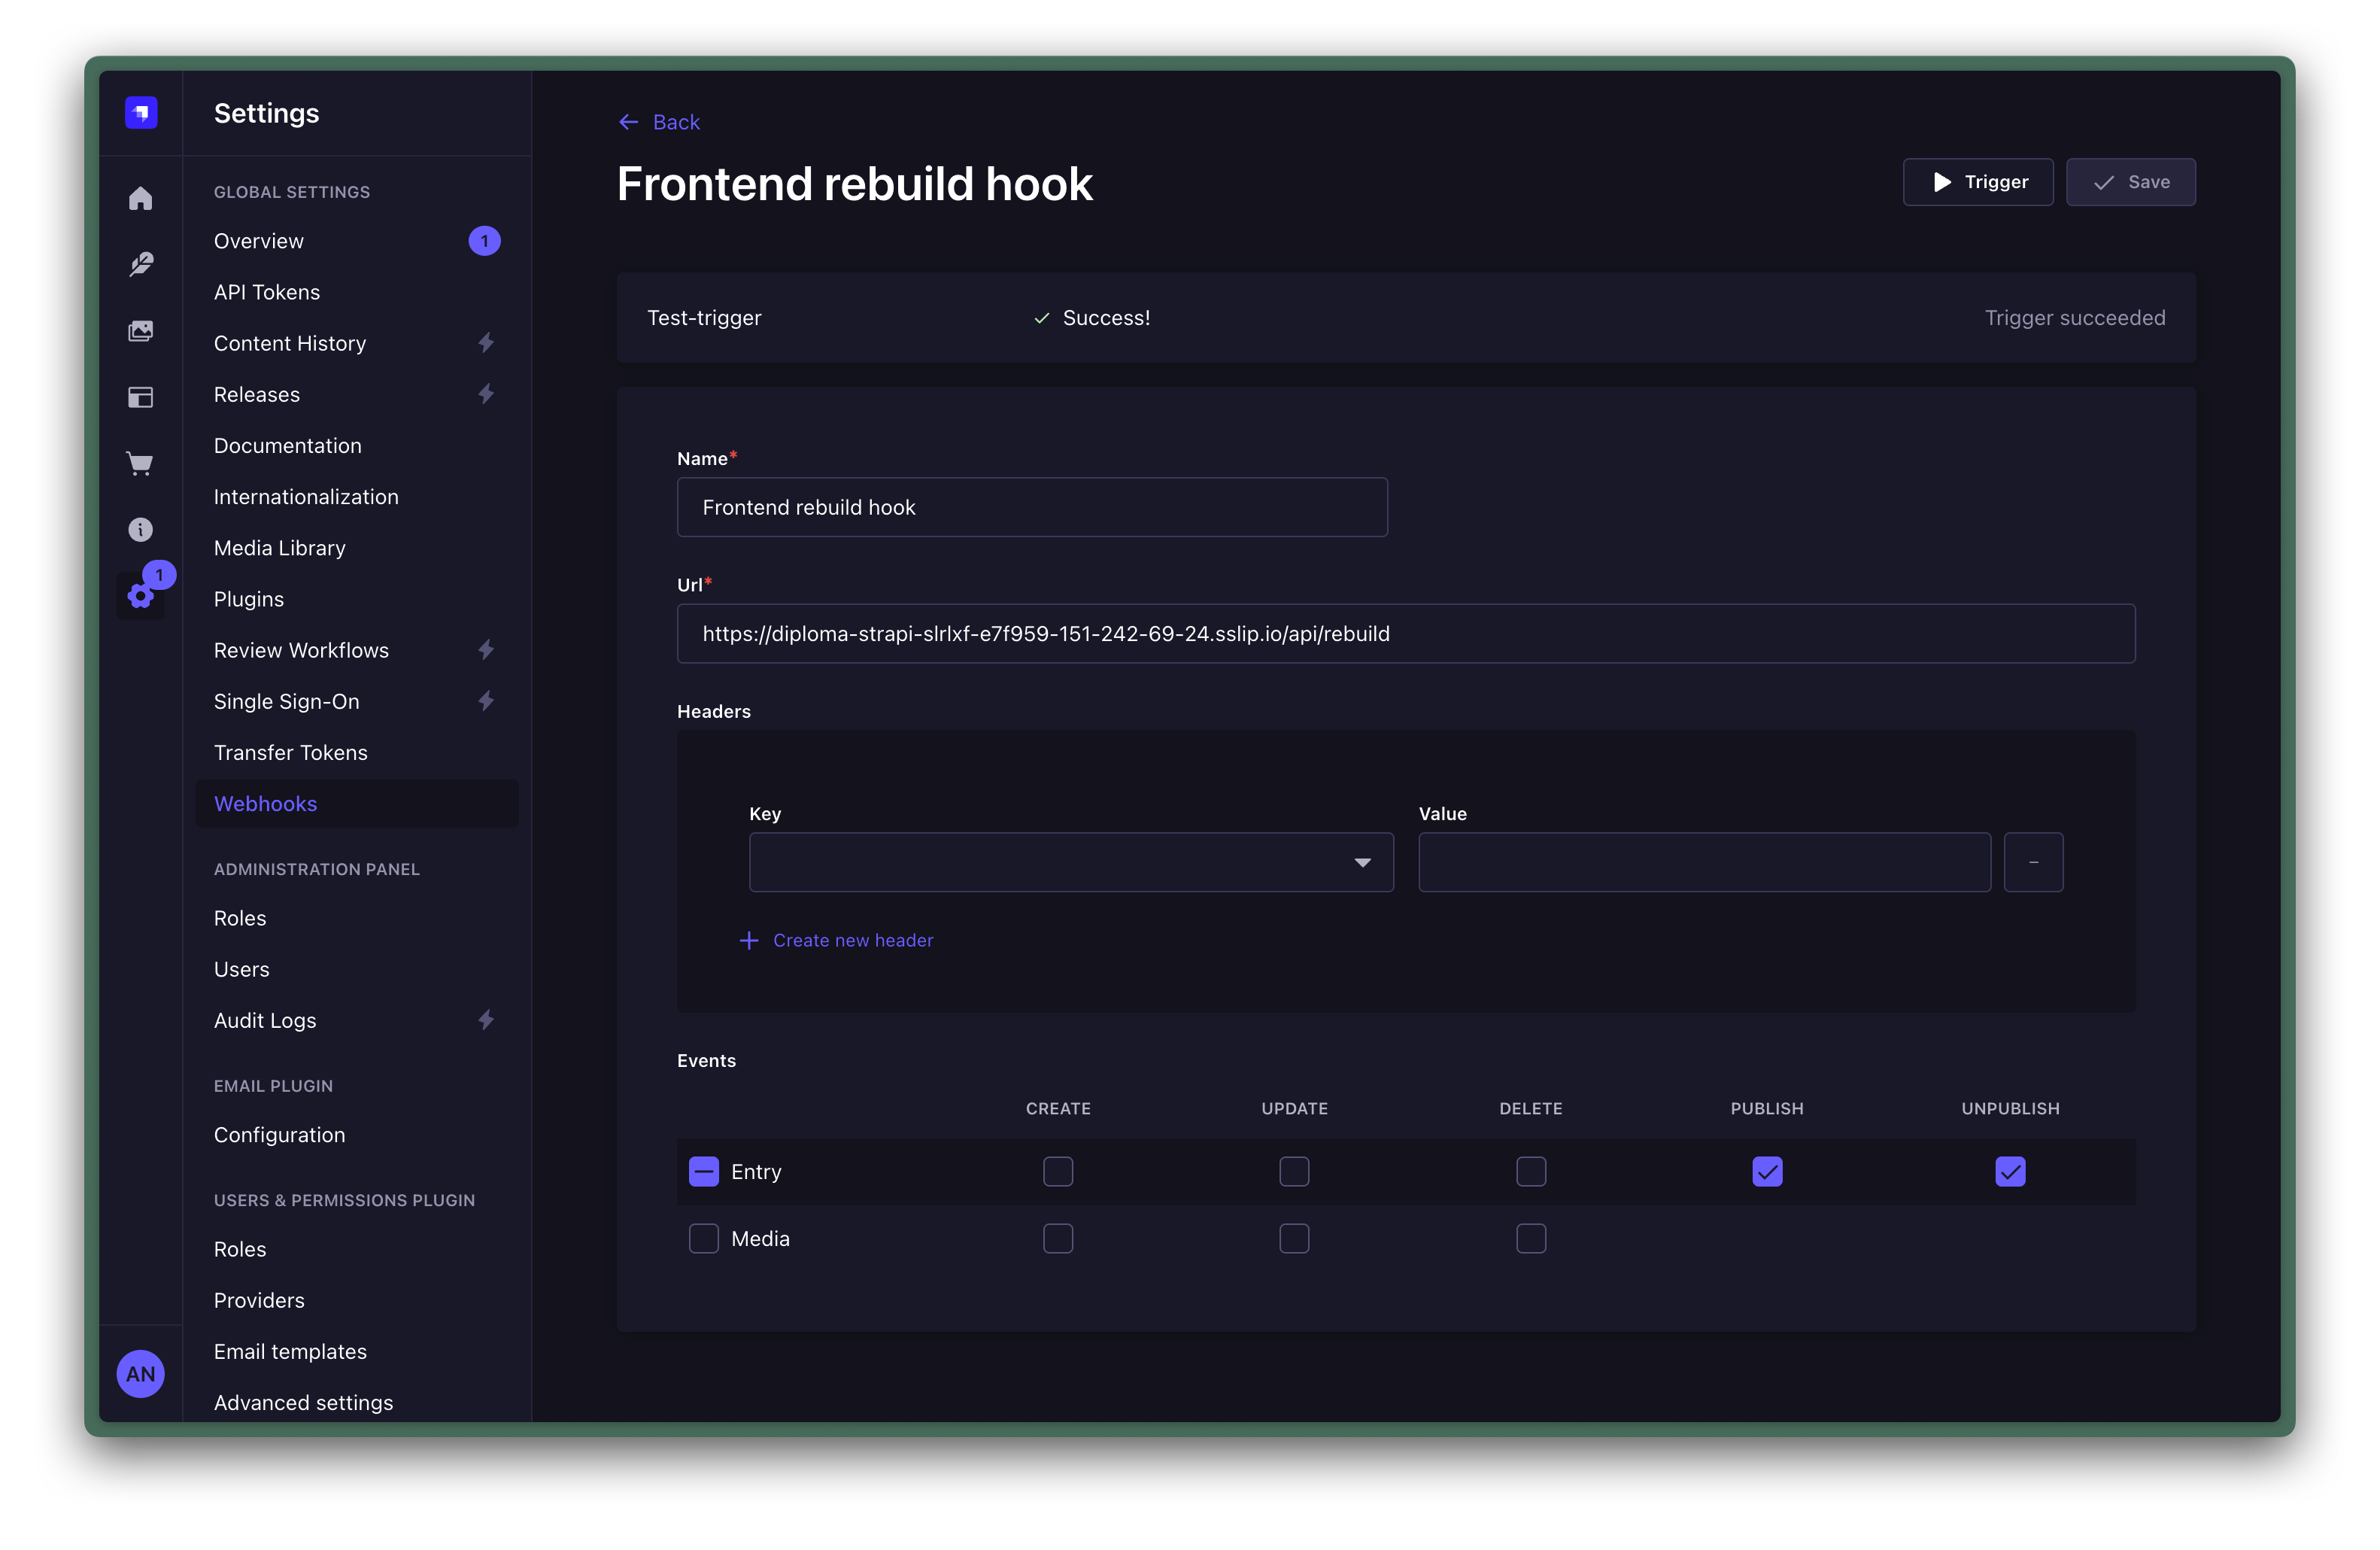
\includegraphics[width=\linewidth]{assets/strapi-images/strapi-webhook.png}
  \caption{Managed rebuild webhook в \texttt{Strapi}: целевой URL и подписка на \texttt{entry.publish}/\texttt{entry.unpublish}}
  \label{fig:chapter2-strapi-webhook}
\end{figure}

На стороне frontend этот сценарий опирается на
\texttt{apps/front/Dockerfile}, где build-stage формирует standalone output
\texttt{Astro}, а runtime-stage запускает серверное приложение на порту \texttt{4321}.
Именно это отдельное frontend \texttt{Docker}-приложение пересобирается и повторно
развертывается
в \texttt{Dokploy}. Публичные маршруты при этом сохраняют модель предварительной сборки,
\texttt{sitemap} генерируется как часть build-контура, а server-side логика используется
точечно для \texttt{preview}. Следовательно, в системе реализована управляемая схема
\texttt{Strapi -> publish -> webhook -> Dokploy rebuild/redeploy -> Astro frontend},
ориентированная на отсутствие ручного запуска frontend-сборки со стороны редактора после
публикации контента.

Локально в рамках работы было подтверждено, что при старте \texttt{Strapi} webhook
автоматически создается в \texttt{strapi\_webhooks}: это было проверено как по логу
\texttt{bootstrap}, так и прямым чтением временной \texttt{sqlite}-базы. Следовательно,
webhook не является скрытой ручной настройкой в интерфейсе, а выступает частью
репозитория и автоматического \texttt{bootstrap}-процесса. Дополнительно 1 июня 2026 года
на внешнем стенде проекта был воспроизведен полный сквозной путь
\texttt{publish/unpublish -> webhook -> Dokploy rebuild/redeploy -> обновление Astro-витрины}.
Следовательно, publication webhook и \texttt{Dokploy}-ориентированный rebuild-контур
подтверждены не только локально на стороне \texttt{CMS}, но и внешним
\texttt{end-to-end} прогоном. При этом сама конфигурация \texttt{Dokploy} остается внешним
платформенным сегментом и не превращается в versioned состояние репозитория.

\subsection{Deployment-архитектура frontend и CMS}

Production-контур системы ориентирован на \texttt{Dokploy}, где frontend и CMS
размещаются как два независимых \texttt{Docker}-приложения. Frontend собирается из
\texttt{apps/front/Dockerfile}: build-stage формирует standalone output \texttt{Astro}, а
runtime-stage запускает серверное приложение на основе \texttt{dist/server/entry.mjs}.
CMS собирается из \texttt{apps/cms/Dockerfile} и исполняет production build
\texttt{Strapi}. Такое разделение соответствует фактической архитектуре проекта:
публичная витрина и CMS обслуживаются независимо и могут обновляться раздельно.
На платформенном уровне это выражается как отдельные сервисы \texttt{astro},
\texttt{strapi} и \texttt{pg} внутри production-окружения
\texttt{Dokploy}, что показано на
рисунке~\ref{fig:chapter2-dokploy-project}.

\begin{figure}[htbp]
  \centering
  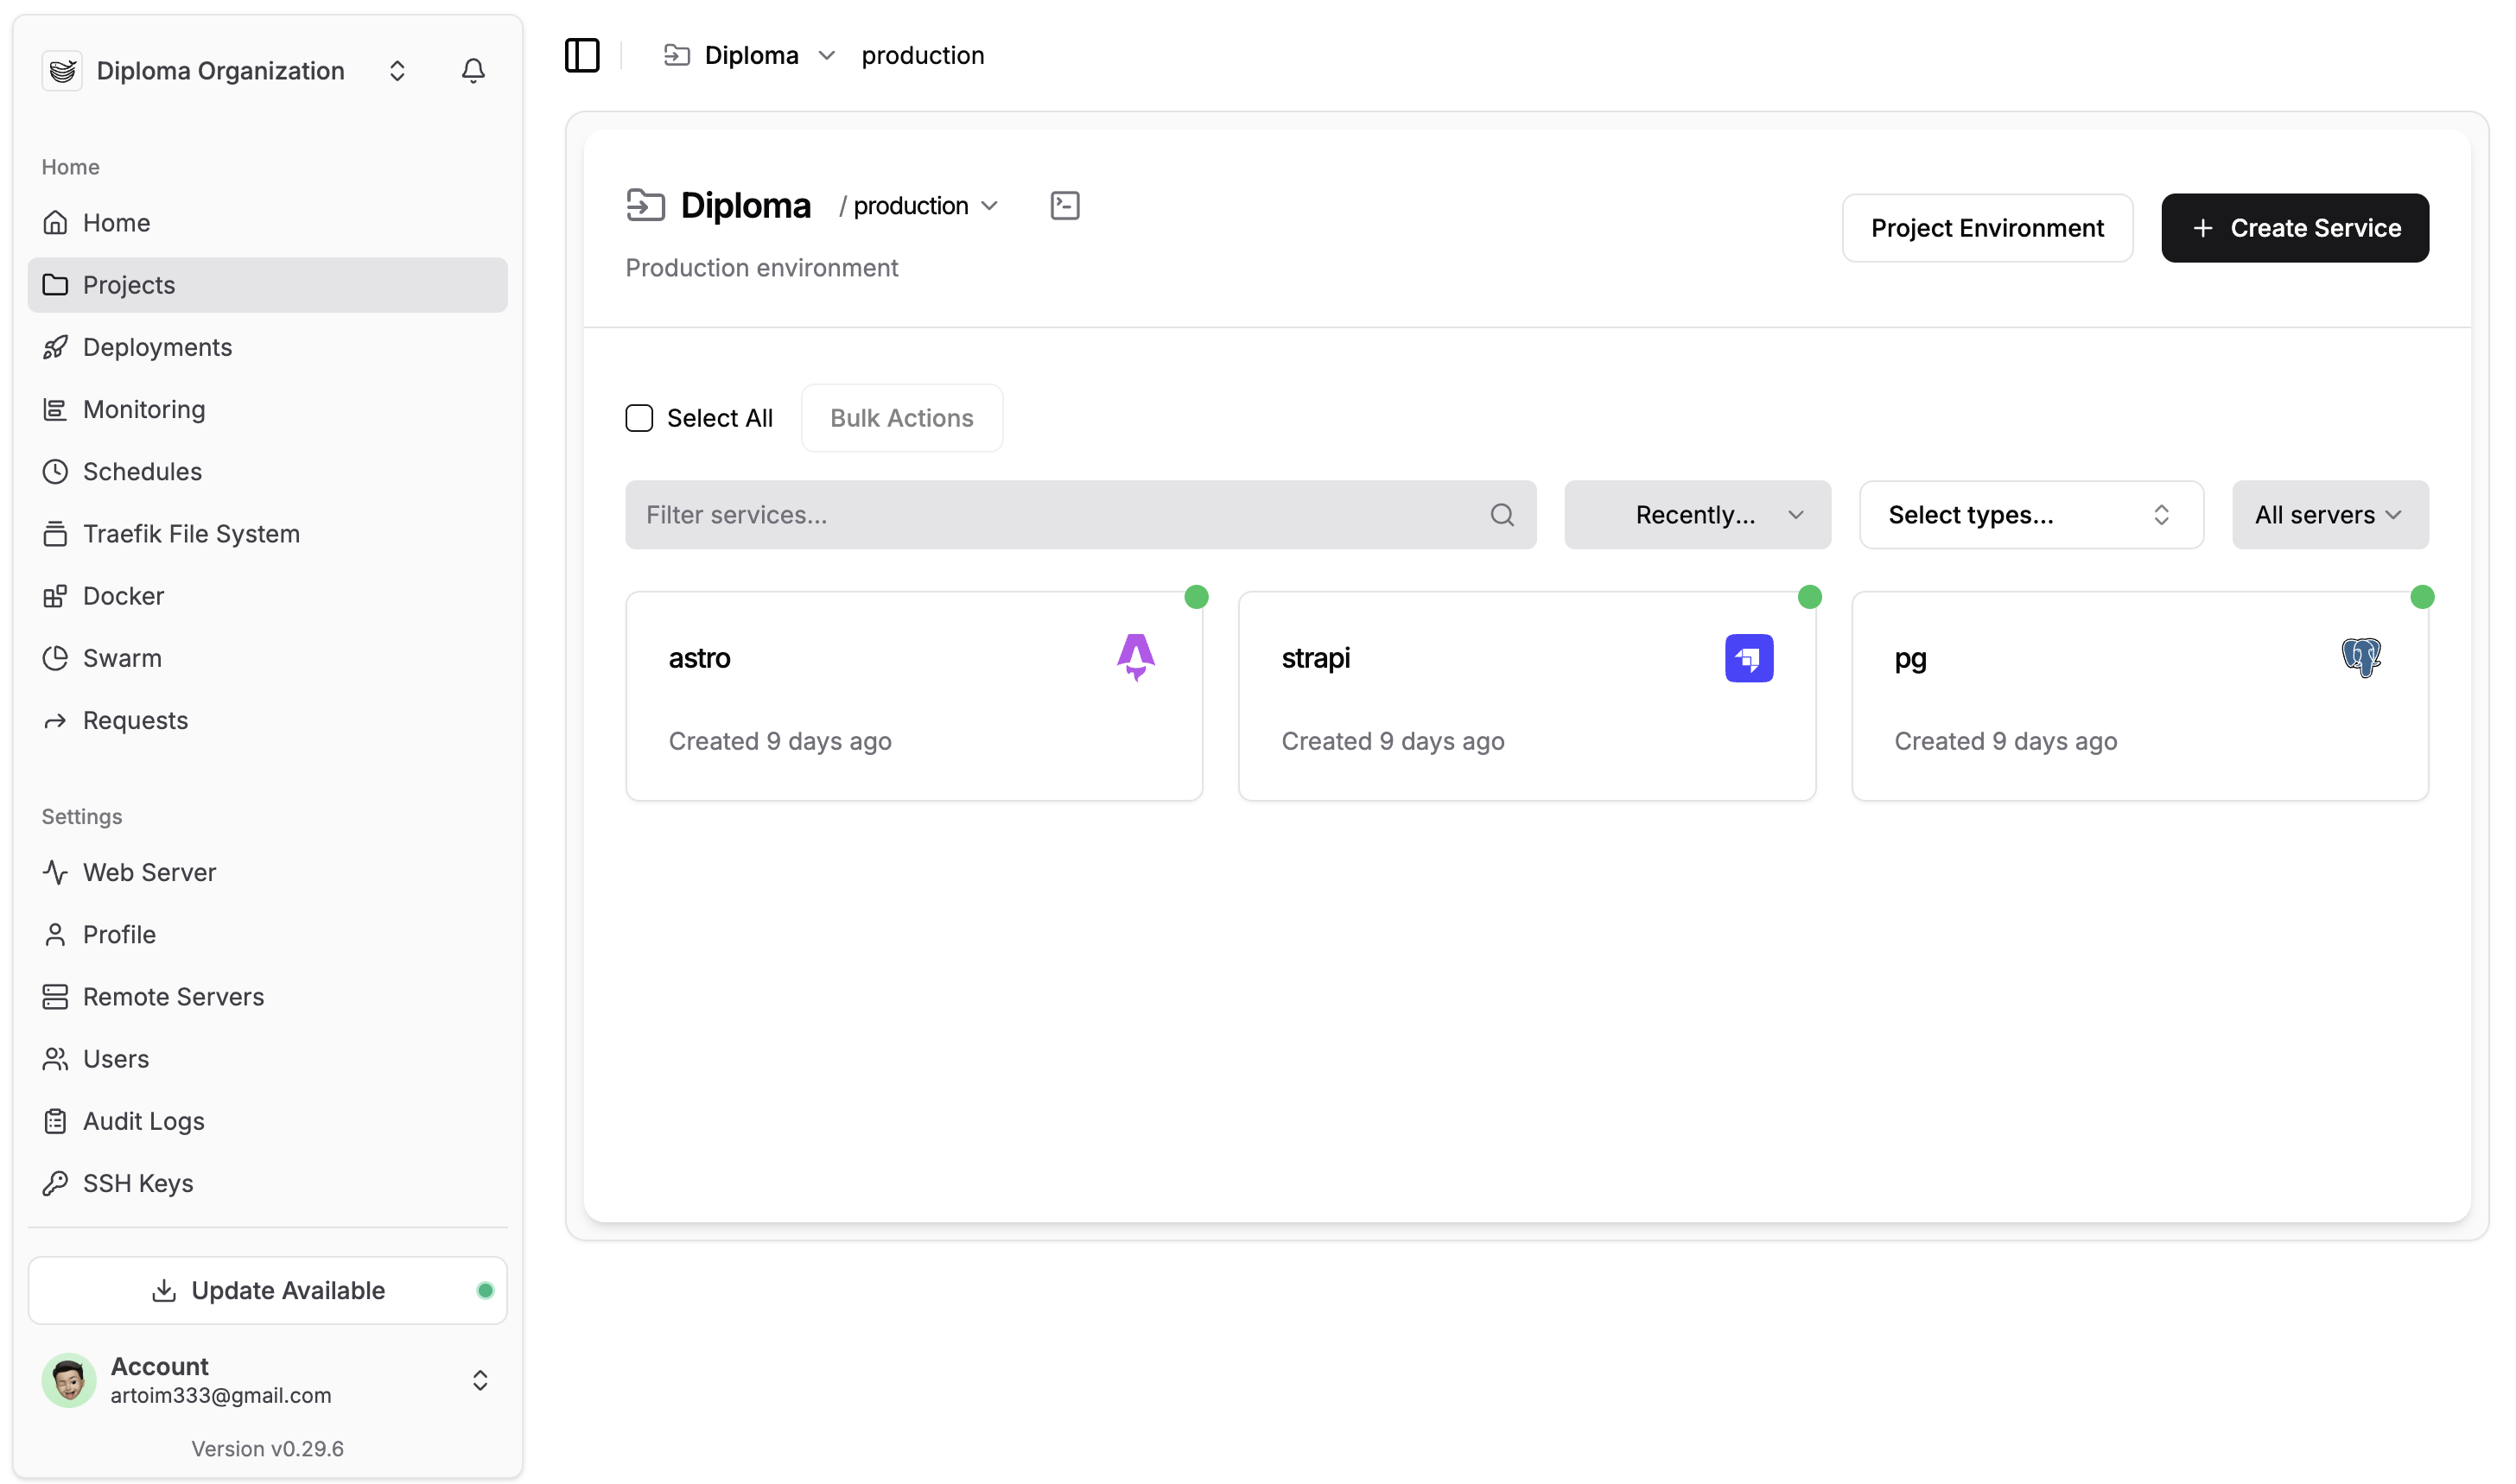
\includegraphics[width=\linewidth]{assets/dokploy/project-home.png}
  \caption{Production-окружение в \texttt{Dokploy} с раздельными сервисами \texttt{astro}, \texttt{strapi} и \texttt{pg}}
  \label{fig:chapter2-dokploy-project}
\end{figure}

Для CMS в репозитории отдельно зафиксирован контур развертывания на базе
\texttt{Docker Compose}. Он включает \texttt{Dockerfile}, \texttt{compose.yml} и
отдельный набор переменных окружения. Внутри этого контура выделяются два сервиса:
\texttt{cms} с приложением \texttt{Strapi} и \texttt{cms-db} с \texttt{PostgreSQL}. Для
медиа-данных предусмотрен отдельный persistent volume \texttt{uploads}. Такой набор
нужен для локальной валидации инфраструктурной схемы и лучше соответствует инженерной
трактовке ВКР, чем неформальный локальный запуск CMS без зафиксированных deployment-
артефактов, поскольку контейнеризация позволяет отделить приложение от инфраструктурного
окружения и воспроизводимо переносить его между средами~\cite{docker-overview}.

С практической точки зрения \texttt{Dokploy} управляет двумя прикладными deployment
unit-ами и одной отдельной зависимостью данных. Для frontend критичны адресные
параметры, доступ к \texttt{CMS} и секреты preview-контура. Для \texttt{CMS}
дополнительно задаются публичный адрес, проксирующий режим, параметры rebuild hook
frontend, настройки подключения к базе данных и собственный набор секретов
\texttt{Strapi}. Тем самым deployment-модель выражается через versioned
\texttt{Dockerfile} и \texttt{env}-контракт, тогда как сам \texttt{Dokploy} хранит
платформенные привязки: public domains, реальные секреты и настройку нативного rebuild
hook.

Платформенная привязка публичного frontend-домена показана на
рисунке~\ref{fig:chapter2-dokploy-astro-domain}: для приложения \texttt{astro}
зафиксированы служебный домен \texttt{Dokploy} и пользовательский домен с \texttt{HTTPS}, что соответствует роли
\texttt{Dokploy} как внешней среды публикации витрины.

\begin{figure}[htbp]
  \centering
  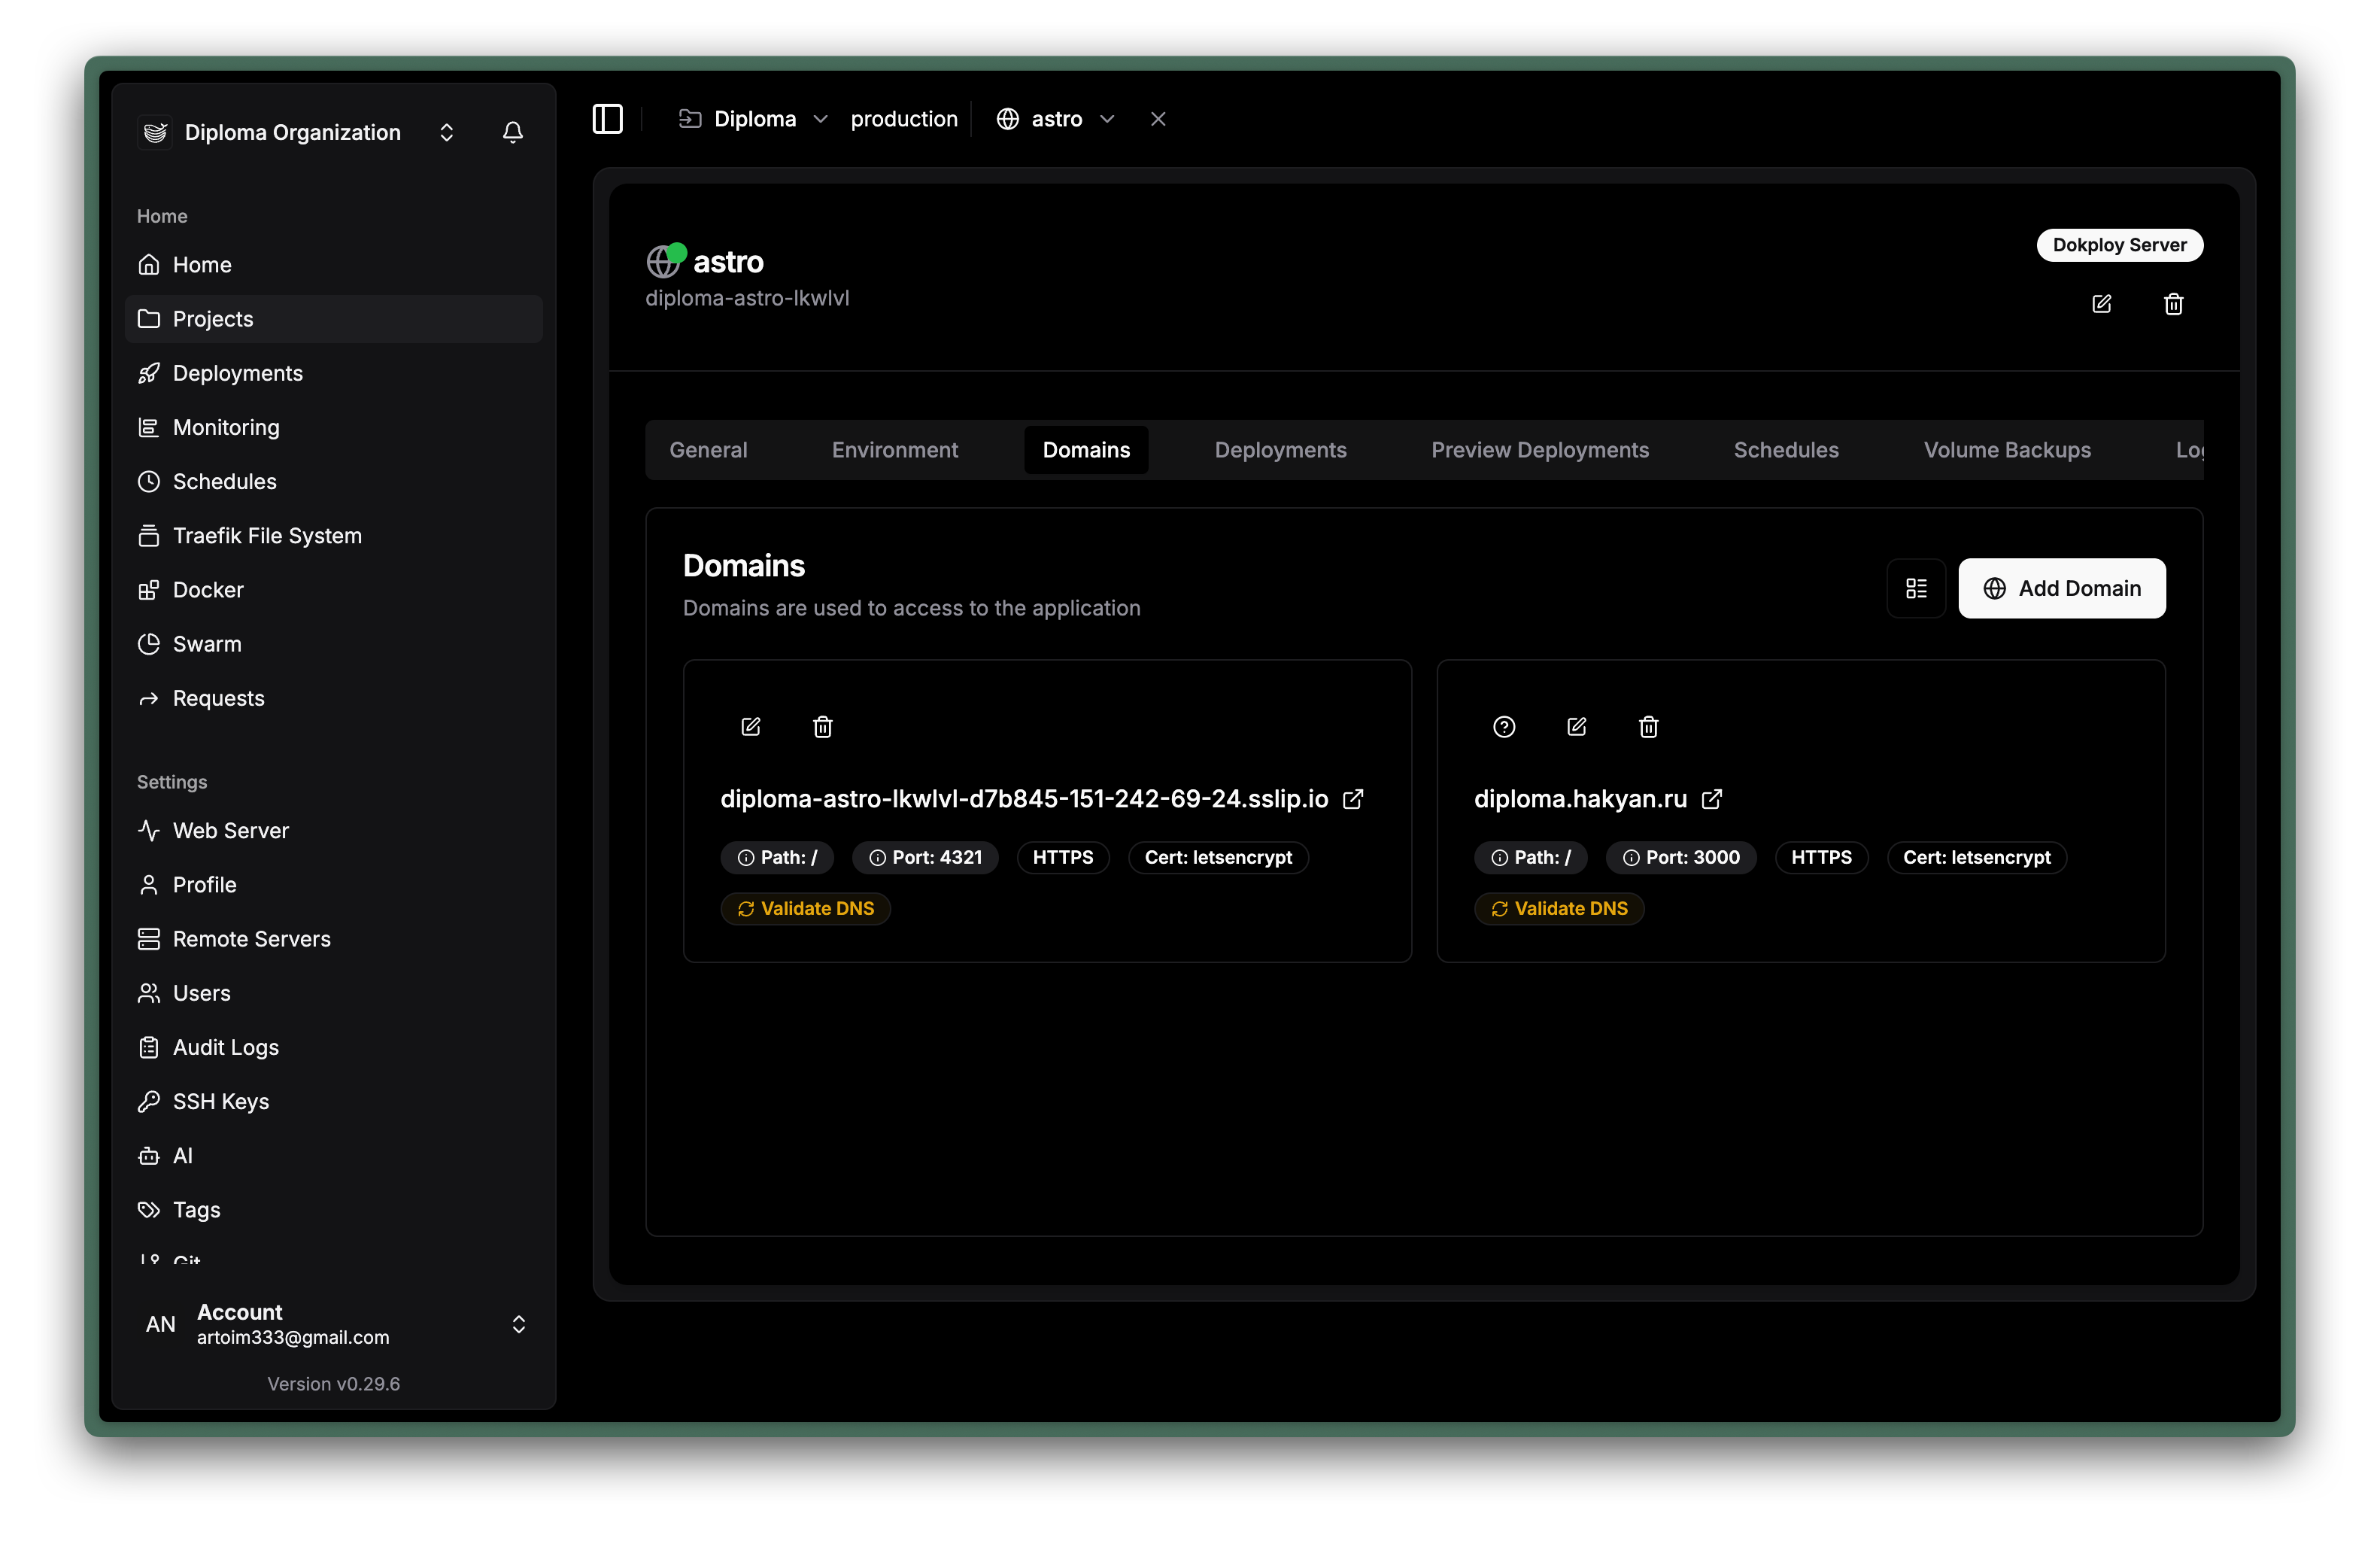
\includegraphics[width=\linewidth]{assets/dokploy/astro-domain.png}
  \caption{Доменная привязка frontend-приложения в \texttt{Dokploy}: служебный домен, пользовательский домен и \texttt{HTTPS}}
  \label{fig:chapter2-dokploy-astro-domain}
\end{figure}

Такое разделение важно и методически. В тексте ВКР контур развертывания описывается не
как устная инструкция по ручному запуску, а как формализованная схема, где application
bundles, инфраструктурные зависимости и публикационный механизм выражены в
репозитории, а внешняя платформа выступает исполнителем этих артефактов.

Локально был подтвержден корректный синтаксис и связность \texttt{compose}-контура через
валидацию итоговой конфигурации. Дополнительно production build самого приложения
\texttt{Strapi} был выполнен успешно; отдельно воспроизводился и production build
frontend с генерацией публичных маршрутов и \texttt{sitemap}. При этом сама platform-state
конфигурация \texttt{Dokploy} относится к внешнему инфраструктурному сегменту. Поэтому
данный результат корректно описывать как \texttt{Dokploy}-ориентированный
deployment-контур, зафиксированный в репозитории, локально подтвержденный сборками
приложений и конфигурационной валидацией, а также дополнительно подтвержденный внешней
\texttt{end-to-end} валидацией на стенде проекта.

\section{Безопасность публичных сценариев}

\subsection{Валидация публичных форм}

Наиболее прикладной публичный сценарий безопасности связан с
формой отклика на вакансию. Для нее реализована клиентская валидация через \texttt{zod} и
\texttt{react-hook-form}. Пользователь обязан указать имя, email и телефон, подтвердить
согласие на обработку персональных данных и прикрепить файл резюме. Для резюме
разрешаются только расширения \texttt{.pdf}, \texttt{.doc} и \texttt{.docx}, а размер
файла ограничен \texttt{10 MB}. Поле сопроводительного письма ограничено по длине.

Дополнительным антиспам-механизмом служит \texttt{honeypot}-поле. При его заполнении
форма не отправляет данные в CMS, а локально завершает сценарий как успешный, что
позволяет отсеивать часть автоматизированных отправок без усложнения пользовательского
пути. После прохождения валидации данные передаются в \texttt{POST /api/vacancy-applications}
как \texttt{FormData} вместе с вложением и служебными полями \texttt{source} и
\texttt{submittedAt}. Тем самым форма отклика уже защищается не только на уровне доступа к
административной панели, но и на уровне публичной точки ввода.

Для маркетинговой формы \texttt{lead-form} используется тот же общий подход защиты, но
с адаптацией под другой прикладной сценарий. На клиенте форма валидируется через
\texttt{zod} и \texttt{react-hook-form}, ограничивает длину имени, компании и описания
задачи, требует подтверждения согласия и использует скрытое \texttt{honeypot}-поле.
В отличие от карьерного сценария отправка выполняется не напрямую в \texttt{Strapi}, а
через frontend-маршрут \texttt{/api/lead-submissions}. Внутри этого маршрута payload
проверяется повторно, после чего данные записываются в отдельную сущность
\texttt{lead-submission} с дополнительной атрибуцией по пути, заголовку, локали и имени
формы. Такое разделение позволяет не смешивать маркетинговые лиды с откликами на вакансии
и не открывать браузеру прямой POST на запись маркетинговой формы в CMS.

\subsection{Публичные справочники карьерного модуля}

Для карьерного раздела в CMS отдельно зафиксированы публичные справочники
\texttt{industry} и \texttt{job-role}. Их роуты ограничены операциями \texttt{find} и
\texttt{findOne} без авторизации, что позволяет frontend загружать значения для фильтров и
карточек вакансий без открытия лишних операций записи через публичный API. Такой подход
сохраняет доступность прикладного сценария поиска вакансий и одновременно минимизирует
поверхность публичного доступа к служебным сущностям.

\subsection{Роли, права и разграничение доступа}

Эксплуатационный контур системы построен на явном разделении ролей, при котором
редактирование, публикация и системное администрирование не смешиваются в одном наборе
полномочий. В административной панели \texttt{Strapi} зафиксированы четыре основные
человеческие роли: \texttt{administrator}, \texttt{marketer/content-manager},
\texttt{editor} и \texttt{hr}. Роль \texttt{administrator} сохраняет полный системный
доступ, включая пользователей, роли, токены, \texttt{webhook}-настройки и общую
конфигурацию \texttt{CMS}. Роль \texttt{marketer/content-manager} отвечает за
маркетинговый контур и может управлять сущностями \texttt{global}, \texttt{home-page},
\texttt{page}, \texttt{article}, \texttt{author} и \texttt{project}, просматривать
\texttt{lead-submission}, выполнять \texttt{preview} и публиковать изменения. Роль
\texttt{editor} ограничена подготовкой маркетинговых черновиков и не получает права
публикации, а роль \texttt{hr} изолирована в пределах карьерного контура и управляет
\texttt{vacancy}, \texttt{industry}, \texttt{job-role} и обработкой
\texttt{vacancy-application}.

Такое разграничение важно не только организационно, но и технически. Публикация
маркетингового контента отделена от его подготовки, поэтому редактор может собирать
материал и проверять его через \texttt{preview}, не раскрывая его на публичной витрине.
Карьерный контур при этом не зависит от маркетинговой роли, а маркетинговый --- от
\texttt{hr}, что уменьшает риск случайного изменения данных вне своей зоны
ответственности. Человеческие роли дополняются техническими каналами доступа:
\texttt{CMS\_API\_TOKEN} используется только серверными маршрутами frontend для записи
\texttt{lead-submission} и \texttt{vacancy-application}, а \texttt{PREVIEW\_SECRET}
используется для чтения черновиков в \texttt{/preview/*}.

На уровне публичного \texttt{Content API} границы доступа дополнительно ужесточены.
Роль \texttt{public} получает только операции \texttt{find}/\texttt{findOne} для
опубликованного контента, а роль \texttt{authenticated} в рамках данной ВКР остается без
прав. Более того, middleware \texttt{enforce-published} принудительно ограничивает
публичные \texttt{GET /api/*} опубликованным состоянием, если запрос не содержит
корректного \texttt{x-preview-secret}. В результате система реализует не декларативную, а
воспроизводимую модель разграничения доступа: браузер не получает write-доступ к
контентным сущностям, черновики не раскрываются через обычный публичный API, а права
публикации остаются только у уполномоченных ролей.

\section{Тестирование}

\subsection{Организация проверки и полученные результаты}

Тестирование разработанной системы было организовано как воспроизводимый контур
приемочной проверки, ориентированный на реальные пользовательские и редакторские
сценарии. Проверка выполнялась в локальном окружении с отдельными процессами
\texttt{Strapi}, runtime frontend и preview-сервера для собранной витрины. Для
повторяемого запуска были зафиксированы workspace-команды smoke-проверки,
мутационного smoke, evidence-сбора и браузерного аудита. Такая организация позволила
перейти от разовой ручной проверки к формализованному набору процедур, который
подтверждает работоспособность ключевых частей \texttt{CMS-first} контура.

Центральным результатом стала автоматизированная smoke-проверка публичной витрины. Она
подтвердила корректность публичных маршрутов, режима предварительного просмотра,
сборочных артефактов и прикладных форм. В контрольной серии проверок от 31 мая 2026 года
read-only прогон завершился без отказов и содержал только одно ожидаемое
предупреждение, связанное с отключенными mutation checks, тогда как мутационный прогон
также прошел без отказов. Тем самым был подтвержден не только факт доступности
маршрутов, но и корректная работа сценариев отправки маркетингового лида и отклика на
вакансию.

В автоматизированной проверке были подтверждены редирект \texttt{/ -> /ru/}, доступность
локализованных маршрутов \texttt{/ru/} и \texttt{/en/}, работа репрезентативных
CMS-страниц, статей, проектов и вакансий, корректность редиректов со старых адресов, а также
наличие \texttt{title}, \texttt{canonical}, \texttt{Open Graph}-метаданных,
\texttt{html[lang]} и основного заголовка \texttt{h1}. Отдельным достижением стало
подтверждение редакторского \texttt{preview}-контура: были воспроизведены отказ по
неверному секрету, корректный переход на опубликованный маршрут для статуса
\texttt{published}, установка \texttt{httpOnly} cookie для статуса \texttt{draft} и
наличие \texttt{robots=noindex, nofollow} на preview-страницах не только для
\texttt{home-page} и \texttt{page}, но и для детальных страниц сущностей
\texttt{article}, \texttt{project} и \texttt{vacancy}.

Существенную часть доказательной базы составили сборочные результаты и результаты на
уровне базы данных. Сборка frontend завершилась успешно и сформировала \texttt{37}
предсобранных HTML-маршрутов, \texttt{sitemap-index.xml} и \texttt{sitemap-0.xml}. Анализ
карты сайта подтвердил наличие маршрутов \texttt{/ru/}, \texttt{/en/}, локализованных детальных страниц
для \texttt{articles/projects}, а также публичных маршрутов \texttt{/vacancies/...}.
SQL-проверки зафиксировали появление новых записей в таблицах
\texttt{lead\_submissions} и \texttt{vacancy\_applications} после мутационного smoke, а
также наличие активного \texttt{Frontend rebuild hook} в таблице
\texttt{strapi\_webhooks}. Это позволяет рассматривать тестирование не только как
проверку интерфейса, но и как подтверждение корректности прикладных записей и
публикационного механизма на уровне данных.

Дополнительно был выполнен браузерный аудит репрезентативных маршрутов через
\texttt{Playwright}. Он подтвердил наличие \texttt{html[lang]} и \texttt{h1},
доступность форм, отсутствие необозначенных элементов форм, \texttt{page errors} и
same-origin runtime/resource failures, а также зафиксировал базовые показатели времени навигации для
\texttt{RU/EN home},
репрезентативной CMS-страницы и детальной вакансии. В совокупности это позволяет
утверждать, что на уровне браузерного исполнения проект продемонстрировал стабильное
поведение как для основной публичной витрины, так и для прикладных публичных сценариев. Сводные
результаты проверки ключевых контуров системы представлены в
таблице~\ref{tab:chapter2-testing-results}.

\begin{longtable}{|L{0.28\linewidth}|L{0.62\linewidth}|}
  \caption{Сводные результаты проверки ключевых контуров системы}
  \label{tab:chapter2-testing-results} \\
  \hline
  \textbf{Контур} & \textbf{Результат проверки} \\
  \hline
  \endfirsthead
  \caption*{Продолжение таблицы~\ref{tab:chapter2-testing-results}} \\
  \hline
  \textbf{Контур} & \textbf{Результат проверки} \\
  \hline
  \endhead
  \hline
  \endfoot
  Публичные маршруты и мультиязычность & Подтверждена доступность маршрутов \texttt{/ru/}, \texttt{/en/}, локализованных CMS-страниц, статей и проектов; устаревшие URL корректно перенаправляются. Основание: автоматизированная smoke-проверка, runtime-проверки, сборочный вывод и \texttt{sitemap}. \\
  \hline
  \texttt{Preview}-сценарии & Подтверждены проверка секрета, установка draft cookie, переход на опубликованный маршрут и применение \texttt{noindex} для preview-страниц. Основание: автоматизированная smoke-проверка и runtime-проверки preview. \\
  \hline
  Публичные формы & Подтверждены server-side валидация, защита по same-origin, отклонение невалидных данных и успешная запись валидных отправок. Основание: mutation smoke и данные SQLite. \\
  \hline
  Сборка и публикационный контур & Подтверждены сформированные предсобранные маршруты, карта сайта и активный \texttt{Frontend rebuild hook}. Основание: frontend build, \texttt{sitemap} и запросы к \texttt{strapi\_webhooks}. \\
  \hline
  Браузерное выполнение & Зафиксировано корректное поведение репрезентативных страниц без \texttt{page errors}, same-origin runtime/resource failures и без необозначенных элементов форм. Основание: браузерный аудит \texttt{Playwright}. \\
  \hline
\end{longtable}

\subsection{Количественные показатели контрольной серии проверок}

Наряду с качественным подтверждением сценариев были зафиксированы количественные
показатели, характеризующие состояние системы в контрольной серии проверок. Они
демонстрируют,
что результат тестирования выражается не только в общем утверждении о работоспособности,
но и в конкретных измеримых значениях, представленных в таблице~\ref{tab:chapter2-testing-metrics}.

\begin{longtable}{|L{0.2\linewidth}|L{0.2\linewidth}|L{0.5\linewidth}|}
  \caption{Ключевые показатели контрольной серии проверок}
  \label{tab:chapter2-testing-metrics} \\
  \hline
  \textbf{Показатель} & \textbf{Значение} & \textbf{Интерпретация} \\
  \hline
  \endfirsthead
  \caption*{Продолжение таблицы~\ref{tab:chapter2-testing-metrics}} \\
  \hline
  \textbf{Показатель} & \textbf{Значение} & \textbf{Интерпретация} \\
  \hline
  \endhead
  \hline
  \endfoot
  Read-only smoke & \texttt{0 failures / 1 warning} & Подтверждены все обязательные маршрутные и preview-проверки; предупреждение связано только с отключенными mutation checks \\
  \hline
  Mutation smoke & \texttt{0 failures / 0 warnings} & Подтверждены успешные сценарии \texttt{lead-submission} и \texttt{vacancy-application} \\
  \hline
  Сборка frontend & \texttt{37} предсобранных HTML-маршрутов & Подтверждена полнота статического контура витрины и локализованных контентных маршрутов \\
  \hline
  Объем \texttt{dist/client} & около \texttt{2.4 MB} & Зафиксирован итоговый размер публичного результата сборки \\
  \hline
  Browser audit & \texttt{0 failures} & Репрезентативные страницы корректно проходят браузерную проверку структуры, форм и ошибок исполнения \\
  \hline
\end{longtable}

\subsection{Практическое значение результатов}

Короткая ручная приемка дополняет автоматизированную проверку и используется как демонстрационный
сценарий на защите. Она включает редирект на \texttt{/ru/}, открытие русской и
английской версии витрины, показ репрезентативной CMS-страницы, запуск
\texttt{preview}-сценария из \texttt{Strapi}, открытие детальной вакансии и проверку
невалидного ввода для маркетинговой и карьерной формы. За счет этого результаты
автоматизированной проверки получают наглядное подтверждение в браузере и демонстрируют,
что проект готов не только к технической верификации, но и к презентации редакторских и
пользовательских сценариев.

Важным итогом этой серии проверок является то, что она подтверждает уже реализованные
достижения проекта: работоспособный двуязычный контур публичной витрины, управляемые
\texttt{SEO}/\texttt{Open Graph}-метаданные, защищенный \texttt{preview}, прикладные
сценарии сбора лидов и откликов, а также публикационную связку между \texttt{Strapi} и
результатом сборки frontend. При этом интерпретация этих результатов должна оставаться
академически корректной: в данной работе подтвержден именно воспроизводимый приемочный и
интеграционный контур проверки, который доказывает зрелость реализованного решения на уровне
ключевых бизнес- и редакторских сценариев.

\section{Выводы по проектной главе}

Реализация проекта образует рабочий \texttt{CMS-first} контур, в котором
\texttt{Strapi} выступает ядром управления контентом, а \texttt{Astro} --- слоем
публикации и рендеринга. В репозитории зафиксированы самостоятельные приложения CMS и
витрины, предметно ориентированная модель данных для статей, проектов, вакансий,
откликов, маркетинговых лидов, глобальных данных и маркетинговых страниц, а также единый
OpenAPI-контур интеграции между backend и frontend.

Практически значимым результатом является перевод главной витрины и
\texttt{pages}-маршрутов в управляемую CMS-модель. Главная страница и маркетинговые
\texttt{slug}-страницы собираются из \texttt{Dynamic Zone}, используют локализованные
маршруты \texttt{ru/en}, получают \texttt{SEO}/\texttt{Open Graph} метаданные из CMS и
поддерживают защищенный \texttt{preview}-сценарий. Дополнительно в системе
функционируют публичные разделы статей, проектов и вакансий; их детальные страницы
используют тот же \texttt{SEO}-контур и тот же механизм preview-метаданных. Карьерный
модуль при этом включает прикладной пользовательский путь от просмотра вакансии до
отправки отклика. Вместе с этим page builder уже поддерживает собственный блок
маркетинговой формы и отдельный сценарий сбора лидов через frontend server route.

Дополнительным результатом стало оформление публикационного контура и контура
развертывания как отдельного инженерного слоя. В репозитории зафиксированы
webhook-связка \texttt{publish/unpublish -> rebuild}, внешний контракт повторной сборки
frontend и \texttt{Docker}-контур CMS. За счет этого вторая глава описывает не только
\texttt{CMS}-модель и маршруты витрины, но и воспроизводимый эксплуатационный процесс
публикации и развертывания.

Таким образом, вторая глава описывает не абстрактный замысел, а реальную
архитектуру и реализованные механизмы управления маркетинговым контентом: разделение CMS и
витрины, предметную модель данных, page builder на основе \texttt{Dynamic Zone},
локализованную витрину первой очереди, управляемый мета-контур, публикационный контур и
контур развертывания, а также безопасный доступ к черновому контенту через
\texttt{preview}.
